% =============================================================================
%  Clasificacion de riesgo crediticio con metodos de kernel (RKHS)
%  Compilar desde la carpeta docs/:   latexmk -pdf report.tex
%
%  Las tablas y los numeros citados en el texto NO estan escritos a mano: se
%  leen de docs/results/ (generado por `python -m rkhs_credit.train`), y las
%  figuras de docs/figures/ (generadas por `python -m rkhs_credit.make_figures`).
% =============================================================================
\documentclass[11pt,a4paper]{article}

\usepackage[T1]{fontenc}
\usepackage[utf8]{inputenc}
\usepackage[spanish,es-tabla,es-noshorthands]{babel}
\usepackage{lmodern}
\usepackage{microtype}
\usepackage[a4paper,margin=2.5cm]{geometry}

\usepackage{amsmath,amssymb,amsthm,mathtools}
\usepackage{graphicx}
\usepackage{booktabs}
\usepackage{enumitem}
\usepackage{xcolor}
\usepackage{caption}
\usepackage{float}      % [H]: tablas exactamente donde se las cita
\usepackage{placeins}   % \FloatBarrier: las figuras no cruzan de seccion
\usepackage{siunitx}
\usepackage{tikz}
\usetikzlibrary{arrows.meta,positioning,fit,calc,babel}
\usepackage[hidelinks]{hyperref}

% El simbolo de "vector de unos" usa el paquete dsfont si esta instalado
% (texlive-fonts-extra); si no, se usa un 1 en negrita.
\IfFileExists{dsfont.sty}%
  {\usepackage{dsfont}\newcommand{\ones}{\mathds{1}}}%
  {\newcommand{\ones}{\mathbf{1}}}

\sisetup{output-decimal-marker={,}, group-minimum-digits=5, exponent-product=\cdot}
\graphicspath{{figures/}}
\captionsetup{font=small,labelfont=bf}
\setlist{itemsep=2pt,topsep=4pt}

% --------------------------------------------------------------- notacion
\newcommand{\R}{\mathbb{R}}
\newcommand{\C}{\mathbb{C}}
\newcommand{\N}{\mathbb{N}}
\newcommand{\X}{\mathcal{X}}
\newcommand{\Hk}{\mathcal{H}}
\newcommand{\dg}{\dagger}                         % daga: traspuesta (conjugada)
\newcommand{\Kc}{\widetilde{K}}                   % matriz de Gram centrada
\newcommand{\inner}[2]{\langle #1,\, #2\rangle}
\newcommand{\norm}[1]{\lVert #1\rVert}
\newcommand{\abs}[1]{\lvert #1\rvert}
\DeclareMathOperator{\tr}{tr}
\DeclareMathOperator{\gen}{gen}
\DeclareMathOperator{\rg}{rg}
\DeclareMathOperator{\sgn}{sgn}
\DeclareMathOperator{\clip}{clip}
\DeclareMathOperator*{\argmax}{arg\,max}
\DeclareMathOperator*{\argmin}{arg\,min}
\newcommand{\good}{\emph{good}}
\newcommand{\bad}{\emph{bad}}
\newcommand{\code}[1]{\texttt{#1}}

\theoremstyle{plain}
\newtheorem{teorema}{Teorema}[section]
\newtheorem{proposicion}[teorema]{Proposición}
\newtheorem{lema}[teorema]{Lema}
\newtheorem{corolario}[teorema]{Corolario}
\theoremstyle{definition}
\newtheorem{definicion}[teorema]{Definición}
\newtheorem{ejemplo}[teorema]{Ejemplo}
\theoremstyle{remark}
\newtheorem{observacion}[teorema]{Observación}

\numberwithin{equation}{section}

% Numeros generados por el script de entrenamiento (\ResSvmCost, etc.).
% Generado por rkhs_credit.train -- no editar a mano.
\newcommand{\ResNSamples}{\num{1000}}
\newcommand{\ResNTrain}{\num{800}}
\newcommand{\ResNTest}{\num{200}}
\newcommand{\ResNTestBad}{\num{60}}
\newcommand{\ResNTestGood}{\num{140}}
\newcommand{\ResNFeatures}{\num{61}}
\newcommand{\ResDataSource}{OpenML}
\newcommand{\ResCostFN}{\num{5}}
\newcommand{\ResCostFP}{\num{1}}
\newcommand{\ResMajorityAuc}{\num{0.500}}
\newcommand{\ResMajorityRecall}{\num{0.000}}
\newcommand{\ResMajorityPrecision}{\num{0.000}}
\newcommand{\ResMajorityAccuracy}{\num{0.700}}
\newcommand{\ResMajorityCost}{\num{300}}
\newcommand{\ResMajorityCostPer}{\num{1.500}}
\newcommand{\ResMajorityFN}{\num{60}}
\newcommand{\ResMajorityFP}{\num{0}}
\newcommand{\ResMajorityTP}{\num{0}}
\newcommand{\ResMajorityTN}{\num{140}}
\newcommand{\ResAlwaysBadAuc}{\num{0.500}}
\newcommand{\ResAlwaysBadRecall}{\num{1.000}}
\newcommand{\ResAlwaysBadPrecision}{\num{0.300}}
\newcommand{\ResAlwaysBadAccuracy}{\num{0.300}}
\newcommand{\ResAlwaysBadCost}{\num{140}}
\newcommand{\ResAlwaysBadCostPer}{\num{0.700}}
\newcommand{\ResAlwaysBadFN}{\num{0}}
\newcommand{\ResAlwaysBadFP}{\num{140}}
\newcommand{\ResAlwaysBadTP}{\num{60}}
\newcommand{\ResAlwaysBadTN}{\num{0}}
\newcommand{\ResLogregAuc}{\num{0.811}}
\newcommand{\ResLogregRecall}{\num{0.883}}
\newcommand{\ResLogregPrecision}{\num{0.427}}
\newcommand{\ResLogregAccuracy}{\num{0.610}}
\newcommand{\ResLogregCost}{\num{106}}
\newcommand{\ResLogregCostPer}{\num{0.530}}
\newcommand{\ResLogregFN}{\num{7}}
\newcommand{\ResLogregFP}{\num{71}}
\newcommand{\ResLogregTP}{\num{53}}
\newcommand{\ResLogregTN}{\num{69}}
\newcommand{\ResSvmAuc}{\num{0.812}}
\newcommand{\ResSvmRecall}{\num{0.917}}
\newcommand{\ResSvmPrecision}{\num{0.414}}
\newcommand{\ResSvmAccuracy}{\num{0.585}}
\newcommand{\ResSvmCost}{\num{103}}
\newcommand{\ResSvmCostPer}{\num{0.515}}
\newcommand{\ResSvmFN}{\num{5}}
\newcommand{\ResSvmFP}{\num{78}}
\newcommand{\ResSvmTP}{\num{55}}
\newcommand{\ResSvmTN}{\num{62}}
\newcommand{\ResKpcaSvmAuc}{\num{0.790}}
\newcommand{\ResKpcaSvmRecall}{\num{0.900}}
\newcommand{\ResKpcaSvmPrecision}{\num{0.415}}
\newcommand{\ResKpcaSvmAccuracy}{\num{0.590}}
\newcommand{\ResKpcaSvmCost}{\num{106}}
\newcommand{\ResKpcaSvmCostPer}{\num{0.530}}
\newcommand{\ResKpcaSvmFN}{\num{6}}
\newcommand{\ResKpcaSvmFP}{\num{76}}
\newcommand{\ResKpcaSvmTP}{\num{54}}
\newcommand{\ResKpcaSvmTN}{\num{64}}
\newcommand{\ResLogregCvCost}{\num{0.516}}
\newcommand{\ResLogregCvCostStd}{\num{0.057}}
\newcommand{\ResLogregCvAuc}{\num{0.778}}
\newcommand{\ResLogregParams}{$C = \num{0.1}$}
\newcommand{\ResSvmCvCost}{\num{0.500}}
\newcommand{\ResSvmCvCostStd}{\num{0.037}}
\newcommand{\ResSvmCvAuc}{\num{0.775}}
\newcommand{\ResSvmParams}{$C = \num{3}$, $\gamma = \num{0.003}$}
\newcommand{\ResKpcaSvmCvCost}{\num{0.486}}
\newcommand{\ResKpcaSvmCvCostStd}{\num{0.032}}
\newcommand{\ResKpcaSvmCvAuc}{\num{0.776}}
\newcommand{\ResKpcaSvmParams}{$C = \num{1}$, $\gamma = \num{0.03}$}
\newcommand{\ResNSupport}{\num{622}}
\newcommand{\ResNFreeSupport}{\num{43}}
\newcommand{\ResNBoundSupport}{\num{579}}
\newcommand{\ResSupportPct}{\num{77.8}}
\newcommand{\ResSmoIter}{\num{1155}}
\newcommand{\ResKktGap}{\num{9.76e-04}}
\newcommand{\ResKktTol}{\num{1e-03}}
\newcommand{\ResBias}{\num{0.380}}
\newcommand{\ResFitSeconds}{\num{0.04}}
\newcommand{\ResSkAgreement}{\num{100.0}}
\newcommand{\ResSkCorr}{\num{1.000000}}
\newcommand{\ResSkMaxDiff}{\num{1.25e-03}}
\newcommand{\ResSkNSupport}{\num{622}}
\newcommand{\ResGramLambdaMax}{\num{736.8}}
\newcommand{\ResGramLambdaMin}{\num{7.30e-07}}
\newcommand{\ResGramRank}{\num{800}}
\newcommand{\ResGramCond}{\num{1.01e+09}}
\newcommand{\ResGramCondJitter}{\num{9.95e+08}}
\newcommand{\ResGramJitter}{\num{1e-08}}
\newcommand{\ResCenteredRank}{\num{799}}
\newcommand{\ResCenteredCond}{\num{1.10e+07}}
\newcommand{\ResSensAuc}{\num{0.812}}
\newcommand{\ResSensRecall}{\num{0.917}}
\newcommand{\ResSensCost}{\num{103}}
\newcommand{\ResSensParams}{$C = \num{3}$, $\gamma = \num{0.003}$}
\newcommand{\ResSensGapSex}{\num{0.128}}
\newcommand{\ResSensGapAge}{\num{0.138}}
\newcommand{\ResSensGapForeign}{\num{0.342}}
\newcommand{\ResNoSensAuc}{\num{0.803}}
\newcommand{\ResNoSensRecall}{\num{0.900}}
\newcommand{\ResNoSensCost}{\num{112}}
\newcommand{\ResNoSensParams}{$C = \num{1}$, $\gamma = \num{0.01}$}
\newcommand{\ResNoSensGapSex}{\num{0.036}}
\newcommand{\ResNoSensGapAge}{\num{0.090}}
\newcommand{\ResNoSensGapForeign}{\num{0.014}}
\newcommand{\ResAgeThreshold}{\num{25}}
\newcommand{\ResRuntime}{\num{54}}


\title{Clasificación de riesgo crediticio con métodos de kernel:\\
       SVM y Kernel PCA en un espacio de Hilbert con núcleo reproductor}
\author{Proyecto \code{RKHS-Model}}
\date{\today}

\begin{document}
\maketitle

\begin{abstract}
\noindent Este documento describe un clasificador de riesgo crediticio construido con métodos
de kernel sobre el conjunto de datos \emph{German Credit} (Statlog): una máquina de vectores
de soporte (SVM) de margen suave, entrenada en su forma dual con el algoritmo SMO, y
\emph{Kernel PCA} para estudiar la estructura no lineal de los datos. Las piezas centrales
(kernels, SMO, Kernel PCA) están implementadas con NumPy/SciPy y validadas contra
\code{scikit-learn}. En el conjunto de test (\ResNTest{} solicitantes) la SVM propia obtiene un
AUC de \ResSvmAuc{} y un costo total de \ResSvmCost{} según la matriz de costos del dataset,
frente a \ResLogregCost{} de la regresión logística, \ResAlwaysBadCost{} de rechazar a todos
y \ResMajorityCost{} del clasificador de clase mayoritaria. El apéndice desarrolla formalmente
la teoría utilizada, con las ecuaciones numeradas que el código fuente cita en sus comentarios.
\end{abstract}

\tableofcontents
\newpage

% =============================================================================
\section{Funcionamiento general}
% =============================================================================

\subsection{El problema}

Un banco recibe una solicitud de crédito descrita por atributos del solicitante y de la
operación (estado de la cuenta, duración y monto del crédito, historial, propósito, empleo,
etc.) y debe decidir si la aprueba. El conjunto \emph{German Credit} (Statlog)
\cite{statlog} contiene \ResNSamples{} solicitudes históricas con 20 atributos (7 numéricos
y 13 categóricos) y una etiqueta: \good{} (el crédito se pagó, 70\,\%) o \bad{} (no se pagó,
30\,\%). Se busca una función $f\colon\X\to\R$ tal que el signo de $f(x)$ prediga la clase;
en todo el proyecto la clase positiva es \bad{} ($y=+1$) y un valor mayor de $f$ significa
\emph{más riesgo}.

Los dos errores posibles no cuestan lo mismo. La documentación del dataset fija la matriz de
costos de la tabla~\ref{tab:costos}: aprobar un crédito que no se paga cuesta \ResCostFN{};
rechazar a un buen pagador cuesta \ResCostFP{}. El objetivo operativo no es entonces acertar
la mayor cantidad de casos, sino minimizar el costo total
\begin{equation}\label{eq:costo-total}
  \text{Costo} \;=\; c_{\mathrm{FN}}\cdot \mathrm{FN} \;+\; c_{\mathrm{FP}}\cdot \mathrm{FP},
  \qquad c_{\mathrm{FN}} = \ResCostFN,\quad c_{\mathrm{FP}} = \ResCostFP,
\end{equation}
donde FN es el número de \bad{} clasificados como \good{} y FP el de \good{} clasificados
como \bad{}.

\begin{table}[H]
  \centering
  \begin{tabular}{lcc}
    \toprule
                 & Predicho \good & Predicho \bad \\
    \midrule
    Real \good   & 0              & \ResCostFP    \\
    Real \bad    & \ResCostFN     & 0             \\
    \bottomrule
  \end{tabular}
  \caption{Matriz de costos del dataset German Credit.}
  \label{tab:costos}
\end{table}

\subsection{Intuición del truco del kernel}

Muchos algoritmos lineales (el hiperplano de margen máximo, el análisis de componentes
principales) solo usan los datos a través de productos internos $x_i^{\dg}x_j$. El
\emph{truco del kernel} consiste en reemplazar ese producto interno por una función
$k(x_i,x_j)$ que es, ella misma, un producto interno en otro espacio:
\begin{equation}\label{eq:truco}
  k(x,y) \;=\; \inner{\varphi(x)}{\varphi(y)}_{\Hk},
\end{equation}
donde $\varphi\colon\X\to\Hk$ lleva cada dato a un espacio de Hilbert $\Hk$ (el
\emph{espacio de características}), posiblemente de dimensión infinita. El algoritmo lineal,
ejecutado en $\Hk$, produce fronteras \emph{no lineales} en el espacio original, y nunca
necesita calcular $\varphi(x)$: le basta la matriz de Gram $K_{ij}=k(x_i,x_j)$, de tamaño
$n\times n$.

\begin{ejemplo}
En $\R^2$, el kernel polinomial $k(x,y)=(x^{\dg}y)^2$ corresponde al mapa
$\varphi(x)=(x_1^2,\ \sqrt2\,x_1x_2,\ x_2^2)$, porque
$(x_1y_1+x_2y_2)^2 = x_1^2y_1^2+2x_1x_2y_1y_2+x_2^2y_2^2 = \varphi(x)^{\dg}\varphi(y)$.
Una elipse en el plano original es un hiperplano en el espacio de características.
La figura~\ref{fig:truco} muestra el caso unidimensional.
\end{ejemplo}

\begin{figure}[htbp]
  \centering
  \begin{tikzpicture}[scale=0.95, >=Stealth,
      good/.style={circle, fill=blue!65!cyan, inner sep=1.7pt},
      bad/.style={regular polygon, regular polygon sides=3, fill=orange!90!red, inner sep=1.2pt}]
    % ----- izquierda: datos en la recta
    \begin{scope}
      \draw[->] (-2.6,0) -- (2.6,0) node[below] {$x$};
      \foreach \x in {-0.8,-0.4,0,0.35,0.75} \node[good] at (\x,0) {};
      \foreach \x in {-2.1,-1.7,-1.35,1.4,1.8,2.2} \fill[orange!90!red] (\x,0) ++(-0.09,-0.08) -- ++(0.18,0) -- ++(-0.09,0.17) -- cycle;
      \node[align=center, font=\small] at (0,-1.0) {En $\R$ ningún umbral\\ separa las clases};
    \end{scope}
    \draw[->, thick] (3.1,0.9) -- node[above, font=\small] {$\varphi(x)=(x,\,x^2)$} (5.5,0.9);
    % ----- derecha: datos sobre la parabola
    \begin{scope}[xshift=8.6cm, yshift=-0.9cm]
      \draw[->] (-2.6,0) -- (2.6,0) node[below] {$x$};
      \draw[->] (0,-0.2) -- (0,3.4) node[left] {$x^2$};
      \draw[gray!60] plot[domain=-2.35:2.35, samples=60] (\x,{0.6*\x*\x});
      \foreach \x in {-0.8,-0.4,0,0.35,0.75} \node[good] at (\x,{0.6*\x*\x}) {};
      \foreach \x in {-2.1,-1.7,-1.35,1.4,1.8,2.2}
        \fill[orange!90!red] (\x,{0.6*\x*\x}) ++(-0.09,-0.08) -- ++(0.18,0) -- ++(-0.09,0.17) -- cycle;
      \draw[thick] (-2.5,0.72) -- (2.5,0.72);
      \node[font=\small, anchor=west] at (0.9,0.42) {hiperplano};
    \end{scope}
  \end{tikzpicture}
  \caption{Truco del kernel en una dimensión. Las clases (círculos y triángulos) no son
  separables en la recta, pero sí lo son por una recta tras aplicar $\varphi(x)=(x,x^2)$,
  cuyo kernel es $k(x,y)=xy+x^2y^2$.}
  \label{fig:truco}
\end{figure}

Dos resultados del apéndice sostienen la construcción. El teorema de Moore--Aronszajn
(teorema~\ref{teo:moore}) asegura que toda función $k$ simétrica y definida positiva es un
producto interno como~\eqref{eq:truco} en un espacio de Hilbert de funciones, su RKHS. El
teorema del representante (teorema~\ref{teo:representante}) asegura que, aunque $\Hk$ tenga
dimensión infinita, la solución óptima es una combinación finita
$f=\sum_{i=1}^n\alpha_i\,k(\cdot,x_i)$ de funciones centradas en los datos: el problema se
reduce a hallar $n$ coeficientes.

\subsection{Por qué SVM y Kernel PCA}

\paragraph{SVM.} La SVM de margen suave busca el hiperplano de $\Hk$ que separa las clases
con el mayor margen posible, tolerando violaciones penalizadas. Es adecuada para este problema
por cuatro razones: (i)~su entrenamiento es un programa cuadrático convexo, con óptimo global
y sin inicialización aleatoria; (ii)~depende de los datos solo a través de $K$, de modo que
cualquier kernel válido sirve sin modificar el algoritmo; (iii)~el costo asimétrico entra de
forma natural como una penalización distinta para cada clase (sección~\ref{sec:svm});
(iv)~la solución es rala: solo los \emph{vectores de soporte} intervienen en la predicción.

\paragraph{Kernel PCA.} Es el análisis de componentes principales realizado en $\Hk$. Mira
la misma geometría que usa la SVM pero sin las etiquetas: el espectro de la matriz de Gram
centrada dice cuántas direcciones del espacio de características tienen varianza apreciable
(la dimensión efectiva que induce el kernel) y sus primeras componentes permiten dibujar los
datos. En el pipeline es además una etapa opcional de reducción de dimensión previa a la SVM.

\paragraph{Relación entre ambos.} Los dos métodos comparten la matriz de Gram y están ligados
por un hecho exacto: entrenar una SVM \emph{lineal} sobre \emph{todas} las componentes de
Kernel PCA equivale a entrenar la SVM con el kernel original
(proposición~\ref{prop:invariancia}). Quedarse con las $q$ primeras componentes es, entonces,
restringir la SVM al subespacio de mayor varianza de $\Hk$.

% =============================================================================
\section{Diagrama de flujo}
% =============================================================================

La figura~\ref{fig:flujo} resume el recorrido de los datos. Todo lo que se \emph{ajusta}
(medias y desvíos de la estandarización, categorías del \emph{one-hot}, autovectores de
Kernel PCA, multiplicadores de la SVM) se calcula únicamente con el conjunto de entrenamiento
o, dentro de la validación cruzada, con la parte de entrenamiento de cada \emph{fold}.

\begin{figure}[htbp]
  \centering
  \begin{tikzpicture}[
      node distance=6mm and 7mm, >=Stealth, font=\small,
      box/.style={draw, rounded corners=2pt, align=center, minimum height=10mm,
                  text width=27mm, fill=gray!8},
      opt/.style={box, dashed, fill=white},
      io/.style={box, fill=blue!8},
      arr/.style={->, thick}]
    \node[io]  (datos) {Datos\\ \code{credit-g} (OpenML)\\ caché local};
    \node[box, right=of datos] (split) {División\\ estratificada\\ 80/20};
    \node[box, right=of split] (prep) {Preprocesamiento\\ \emph{one-hot} + estandarización};
    \node[box, right=of prep] (gram) {Matriz de Gram\\ $K_{ij}=k(x_i,x_j)$};
    \node[opt, below=11mm of gram] (kpca) {Kernel PCA\\ $\Kc=HKH$, autovalores, proyección};
    \node[box, left=of kpca] (svm) {SVM dual / SMO\\ pesos por clase,\\ sesgo $b$};
    \node[box, left=of svm] (eval) {Evaluación\\ AUC, \emph{recall}, costo, subgrupos};
    \node[io, left=of eval] (fig) {Tablas y figuras\\ \code{docs/results}\\ \code{docs/figures}};
    \node[box, below=9mm of svm, text width=78mm, minimum height=8mm, fill=orange!10] (cv)
      {Validación cruzada estratificada (5 \emph{folds}) sobre $(C,\gamma)$};
    \node[io, above=7mm of prep, text width=78mm, minimum height=7mm] (yaml)
      {\code{configs/default.yaml}: hiperparámetros, rutas y semilla};

    \draw[arr] (datos) -- (split);
    \draw[arr] (split) -- node[above, font=\scriptsize] {train} (prep);
    \draw[arr] (prep) -- (gram);
    \draw[arr, dashed] (gram) -- node[right, font=\scriptsize] {opcional} (kpca);
    \draw[arr, dashed] (kpca) -- (svm);
    \draw[arr] (gram.south west) -- (svm.north east);
    \draw[arr] (svm) -- (eval);
    \draw[arr] (eval) -- (fig);
    \draw[arr] (split.south) |- ($(eval.north)+(0,4mm)$) -- node[right, font=\scriptsize, pos=0.4] {test} (eval.north);
    \draw[arr] (cv.north) -- (svm.south);
    \draw[arr] (cv.west) -| (eval.south);
    \draw[arr, gray] (yaml) -- (prep);
  \end{tikzpicture}
  \caption{Flujo de datos del proyecto. Los bloques de trazos son opcionales (se activan con
  \code{kpca.enabled}). La validación cruzada repite el tramo preprocesamiento--SVM--evaluación
  dentro del conjunto de entrenamiento para elegir los hiperparámetros.}
  \label{fig:flujo}
\end{figure}

\begin{enumerate}
  \item \textbf{Datos.} \code{fetch\_openml("credit-g", version=1)} descarga la tabla una vez
        y se guarda como CSV en \code{data/}. Las corridas de este informe usaron como fuente
        \ResDataSource.
  \item \textbf{División.} 80\,\% entrenamiento (\ResNTrain{} filas) y 20\,\% test
        (\ResNTest{} filas), estratificada por clase y con semilla fija.
  \item \textbf{Preprocesamiento.} Los atributos numéricos se estandarizan y los categóricos
        se codifican \emph{one-hot}; resultan \ResNFeatures{} variables.
  \item \textbf{Matriz de Gram.} El kernel configurado se evalúa de forma vectorizada; la
        matriz se simetriza y, para la SVM, se le suma un \emph{jitter} en la diagonal.
  \item \textbf{Kernel PCA (opcional).} Centrado $\Kc=HKH$, diagonalización, normalización y
        proyección (sección~\ref{sec:kpca}).
  \item \textbf{SVM/SMO.} Se resuelve el dual con pesos por clase tomados de la matriz de
        costos (secciones~\ref{sec:svm} y~\ref{sec:smo}).
  \item \textbf{Evaluación.} AUC-ROC, \emph{recall} y precisión de la clase \bad, matriz de
        confusión, costo~\eqref{eq:costo-total} y métricas por subgrupo.
  \item \textbf{Tablas y figuras.} Se escriben en \code{docs/results} y \code{docs/figures},
        de donde las toma este documento.
\end{enumerate}

% =============================================================================
\section{Arquitectura del código}
% =============================================================================

El paquete \code{rkhs\_credit} (carpeta \code{src/}) está dividido en módulos chicos con una
sola responsabilidad (tabla~\ref{tab:modulos}). La figura~\ref{fig:modulos} muestra cómo
dependen entre sí: las tres piezas matemáticas (\code{kernels}, \code{svm}, \code{kpca}) no
conocen ni los datos ni la configuración, y solo \code{pipeline} convierte el YAML en objetos.

\begin{table}[H]
  \centering
  \small
  \begin{tabular}{@{}lp{0.74\textwidth}@{}}
    \toprule
    Módulo & Responsabilidad \\
    \midrule
    \code{numerics}   & Estabilidad numérica: simetrización, \emph{jitter}, centrado $HKH$,
                        recorte del espectro, número de condición. \\
    \code{kernels}    & Clase base abstracta \code{Kernel}; kernels lineal, RBF y polinomial;
                        suma, producto y escalado; registro por nombre para el YAML. \\
    \code{svm}        & Función \code{smo} (optimizador del dual) y estimador \code{KernelSVM}
                        (pesos por clase, sesgo, \code{decision\_function}, \code{predict}). \\
    \code{kpca}       & \code{KernelPCA}: ajuste, proyección de puntos nuevos, espectro. \\
    \code{data}       & Descarga y caché del dataset, división estratificada,
                        preprocesador tabular, grupos de atributos sensibles. \\
    \code{pipeline}   & \code{CreditPipeline} (preprocesamiento $\to$ Kernel PCA opcional
                        $\to$ SVM), \emph{baselines} y construcción desde la configuración. \\
    \code{tuning}     & Validación cruzada estratificada y búsqueda en grilla. \\
    \code{evaluation} & Matriz de costos, métricas globales y por subgrupo. \\
    \code{reporting}  & Escritura de \code{metrics.json}, tablas y macros de \LaTeX. \\
    \code{plots}      & Una función por figura; no cargan datos ni ajustan modelos. \\
    \code{config}     & Lectura del YAML y claves anidadas con puntos
                        (\code{svm.kernel.gamma}). \\
    \code{train}, \code{make\_figures} & Puntos de entrada por línea de comandos. \\
    \bottomrule
  \end{tabular}
  \caption{Módulos del paquete \code{rkhs\_credit}.}
  \label{tab:modulos}
\end{table}

\begin{figure}[htbp]
  \centering
  \begin{tikzpicture}[
      >=Stealth, font=\small\ttfamily,
      m/.style={draw, rounded corners=2pt, minimum height=7mm, minimum width=21mm, fill=gray!8},
      core/.style={m, fill=blue!10},
      cli/.style={m, fill=orange!12},
      dep/.style={->, gray!70!black}]
    \node[core] (numerics) at (0,0) {numerics};
    \node[core] (kernels) at (0,1.5) {kernels};
    \node[core] (svm) at (-2.0,3.0) {svm};
    \node[core] (kpca) at (2.0,3.0) {kpca};
    \node[m] (data) at (5.2,3.0) {data};
    \node[m] (evaluation) at (-5.2,3.0) {evaluation};
    \node[m] (config) at (5.2,4.5) {config};
    \node[m] (pipeline) at (0,4.5) {pipeline};
    \node[m] (tuning) at (-3.2,6.0) {tuning};
    \node[m] (reporting) at (-6.0,6.0) {reporting};
    \node[m] (plots) at (5.2,6.0) {plots};
    \node[cli] (train) at (-2.2,7.5) {train};
    \node[cli] (figures) at (3.2,7.5) {make\_figures};

    \draw[dep] (kernels) -- (numerics);
    \draw[dep] (svm) -- (kernels);
    \draw[dep] (kpca) -- (kernels);
    \draw[dep] (svm) to[bend right=40] (numerics);
    \draw[dep] (kpca) to[bend left=40] (numerics);
    \draw[dep] (pipeline) -- (svm);
    \draw[dep] (pipeline) -- (kpca);
    \draw[dep] (pipeline) -- (data);
    \draw[dep] (pipeline) -- (evaluation);
    \draw[dep] (tuning) -- (pipeline);
    \draw[dep] (tuning) -- (evaluation);
    \draw[dep] (tuning) to[bend left=12] (config);
    \draw[dep] (train) -- (tuning);
    \draw[dep] (train) -- (pipeline);
    \draw[dep] (train) -- (reporting);
    \draw[dep] (figures) -- (plots);
    \draw[dep] (figures) -- (pipeline);
    \draw[dep] (figures) -- (config);
  \end{tikzpicture}
  \caption{Dependencias principales entre módulos (una flecha $A\to B$ significa
  «$A$ importa $B$»). En azul, las piezas matemáticas implementadas con NumPy/SciPy;
  en naranja, los puntos de entrada.}
  \label{fig:modulos}
\end{figure}

\paragraph{Decisiones de diseño.} Cada una se justifica brevemente:
\begin{enumerate}
  \item \textbf{Kernels como objetos sin estado y componibles.} Un kernel guarda sus
        hiperparámetros y expone \code{gram(X, Y)}; la suma y el producto se construyen con
        \code{k1 + k2} y \code{k1 * k2}. La clausura bajo esas operaciones es un teorema
        (sección~\ref{sec:schur}), no una convención. Agregar un kernel es escribir una
        subclase y registrarla; ningún otro módulo cambia.
  \item \textbf{SMO con el paso analítico de Platt y selección del par de máxima violación.}
        La actualización de dos multiplicadores es exactamente la de Platt
        \cite{platt1998}. Para \emph{elegir} el par se usa la regla de Keerthi et
        al.~\cite{keerthi2001} en lugar de las heurísticas originales: es determinista, su
        criterio de parada es literalmente «las condiciones KKT se cumplen con tolerancia
        $\tau$» y evita mantener un umbral $b$ durante la optimización. Es la misma familia
        de algoritmo que usa LIBSVM \cite{libsvm}, lo que facilita la validación contra
        \code{scikit-learn}.
  \item \textbf{Matriz de Gram completa en memoria.} Con $n\approx 10^3$ ocupa pocos MB y
        vuelve trivial cada iteración. No se implementan caché de columnas ni
        \emph{shrinking}: se priorizó la claridad (sección~\ref{sec:limitaciones}).
  \item \textbf{Sesgo calculado al final} a partir de los vectores de soporte libres
        (ecuación~\eqref{eq:bias-free-sv}), promediando para reducir el error numérico.
  \item \textbf{El costo entra dos veces:} en el entrenamiento, como pesos por clase
        $C_i=C\,w_{y_i}$ con $w_{\bad}=\ResCostFN$ y $w_{\good}=\ResCostFP$; y en la
        selección de hiperparámetros, que minimiza el costo medio de validación cruzada.
  \item \textbf{Kernel PCA por diagonalización densa} de $\Kc$ con \code{scipy.linalg.eigh}.
        El PCA lineal de las figuras es el mismo código con el kernel lineal.
  \item \textbf{Preprocesador propio y explícito} (\code{TabularPreprocessor}): deja a la
        vista que las estadísticas salen solo del conjunto con el que se llama a \code{fit}.
  \item \textbf{Configuración como diccionario} leído del YAML; las grillas de validación
        cruzada nombran los hiperparámetros con claves punteadas, de modo que buscar sobre
        otro parámetro no requiere tocar código.
  \item \textbf{Resultados como macros de \LaTeX}: ningún número de este informe está
        escrito a mano.
  \item \textbf{Fuente de datos alternativa.} Si OpenML no responde, el cargador recurre al
        archivo original de UCI y lo decodifica al mismo formato (se verificó que ambas
        fuentes producen tablas idénticas). Es un agregado respecto del pedido original,
        desactivable con \code{data.fallback\_url: null}.
\end{enumerate}

% =============================================================================
\section{Resultados}\label{sec:resultados}
% =============================================================================

\subsection{Protocolo}

Los hiperparámetros se eligieron por validación cruzada estratificada de 5 \emph{folds}
sobre el conjunto de entrenamiento, minimizando el costo medio por
solicitante~\eqref{eq:costo-total}; el conjunto de test se usó una sola vez, al final. Los
modelos comparados son: (a)~el clasificador trivial de clase mayoritaria, que aprueba a
todos; (b)~el clasificador trivial que rechaza a todos, que es el mejor clasificador
constante bajo esta matriz de costos; (c)~una regresión logística con los mismos pesos por
clase; (d)~la SVM propia con kernel RBF; (e)~Kernel PCA seguido de una SVM lineal. Toda la
corrida (validación cruzada incluida) tarda alrededor de \ResRuntime{} segundos en una CPU
común.

\subsection{Selección de hiperparámetros}

\begin{table}[H]
  \centering
  \small
  \begin{tabular}{llrr}
\toprule
Modelo & Hiperparámetros elegidos & Costo CV (media $\pm$ desvío) & AUC CV \\
\midrule
Regresión logística & $C = \num{0.1}$ & \num{0.516} $\pm$ \num{0.057} & \num{0.778} \\
SVM propia (SMO) & $C = \num{3}$, $\gamma = \num{0.003}$ & \num{0.500} $\pm$ \num{0.037} & \num{0.775} \\
Kernel PCA + SVM lineal & $C = \num{1}$, $\gamma = \num{0.03}$ & \num{0.486} $\pm$ \num{0.032} & \num{0.776} \\
\bottomrule
\end{tabular}

  \caption{Hiperparámetros elegidos por validación cruzada y su desempeño medio en los
  \emph{folds} de validación (costo por solicitante).}
  \label{tab:cv}
\end{table}

\begin{figure}[htbp]
  \centering
  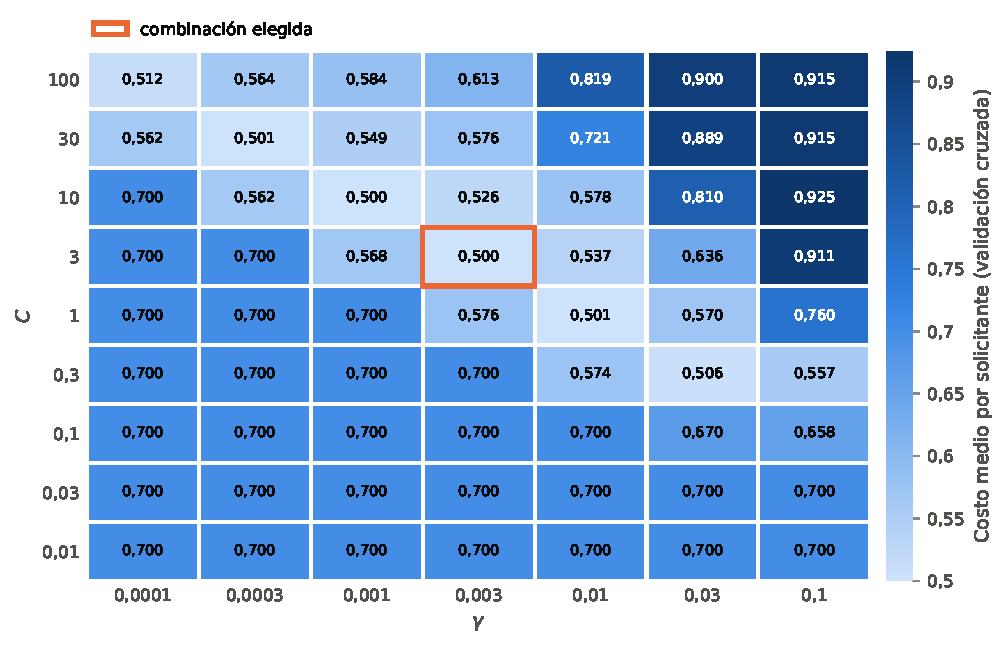
\includegraphics[width=0.78\textwidth]{cv_heatmap}
  \caption{Costo medio de validación cruzada de la SVM con kernel RBF sobre la grilla
  $(C,\gamma)$. El valor \num{0.700} corresponde a modelos que rechazan a todos.}
  \label{fig:heatmap}
\end{figure}

La figura~\ref{fig:heatmap} muestra una estructura clara: las mejores combinaciones forman
una diagonal a lo largo de la cual $C\gamma$ es aproximadamente constante, y todas tienen
prácticamente el mismo costo ($\approx\ResSvmCvCost$). No es casual. Para $\gamma$ pequeño,
$e^{-\gamma\norm{x-y}^2}\approx 1-\gamma\norm{x-y}^2$, y sobre los vectores $\beta$ con
$\ones^{\dg}\beta=0$ (la restricción del dual) vale
$\beta^{\dg}K_{\mathrm{RBF}}\,\beta \approx 2\gamma\,\beta^{\dg}XX^{\dg}\beta$: la SVM
gaussiana con parámetros $(C,\gamma)$ se comporta como una SVM \emph{lineal} con constante
$C_{\mathrm{lin}}=2\gamma C$ \cite{keerthilin2003}. La combinación elegida
(\ResSvmParams) corresponde a $C_{\mathrm{lin}}\approx\ResSvmLinearC$. La conclusión honesta
es que, en este dataset, el modelo seleccionado es casi lineal: la no linealidad del kernel
no aporta una mejora medible, y aumentar $\gamma$ (esquina superior derecha) sobreajusta.

\FloatBarrier
\subsection{Comparación en test}

\begin{table}[H]
  \centering
  \small
  \setlength{\tabcolsep}{4pt}
  \begin{tabular}{lrrrrrrrr}
\toprule
Modelo & AUC & Recall \emph{bad} & Precisión \emph{bad} & Exactitud & FN & FP & Costo & Costo/solic. \\
\midrule
Trivial: clase mayoritaria (aprobar a todos) & \num{0.500} & \num{0.000} & \num{0.000} & \num{0.700} & \num{60} & \num{0} & \num{300} & \num{1.500} \\
Trivial: rechazar a todos & \num{0.500} & \num{1.000} & \num{0.300} & \num{0.300} & \num{0} & \num{140} & \num{140} & \num{0.700} \\
Regresión logística & \num{0.811} & \num{0.883} & \num{0.427} & \num{0.610} & \num{7} & \num{71} & \num{106} & \num{0.530} \\
SVM propia (SMO) & \num{0.812} & \num{0.917} & \num{0.414} & \num{0.585} & \num{5} & \num{78} & \num{103} & \num{0.515} \\
Kernel PCA + SVM lineal & \num{0.790} & \num{0.900} & \num{0.415} & \num{0.590} & \num{6} & \num{76} & \num{106} & \num{0.530} \\
\bottomrule
\end{tabular}

  \caption{Desempeño en el conjunto de test (\ResNTest{} solicitantes: \ResNTestGood{}
  \good{} y \ResNTestBad{} \bad). \emph{Recall} y precisión se refieren a la clase \bad.
  FN: \bad{} clasificados como \good; FP: \good{} clasificados como \bad.
  Costo $=\ResCostFN\cdot\mathrm{FN}+\ResCostFP\cdot\mathrm{FP}$; la última columna es el
  costo por solicitante.}
  \label{tab:modelos}
\end{table}

\begin{table}[H]
  \centering
  \small
  \begin{minipage}{0.47\textwidth}\centering
    \begin{tabular}{lrr}
\toprule
 & Predicho \emph{good} & Predicho \emph{bad} \\
\midrule
Real \emph{good} & \num{62} & \num{78} \\
Real \emph{bad} & \num{5} & \num{55} \\
\bottomrule
\end{tabular}
\\[2pt]
    SVM propia
  \end{minipage}\hfill
  \begin{minipage}{0.47\textwidth}\centering
    \begin{tabular}{lrr}
\toprule
 & Predicho \emph{good} & Predicho \emph{bad} \\
\midrule
Real \emph{good} & \num{69} & \num{71} \\
Real \emph{bad} & \num{7} & \num{53} \\
\bottomrule
\end{tabular}
\\[2pt]
    Regresión logística
  \end{minipage}
  \caption{Matrices de confusión en test.}
  \label{tab:confusion}
\end{table}

\begin{figure}[htbp]
  \centering
  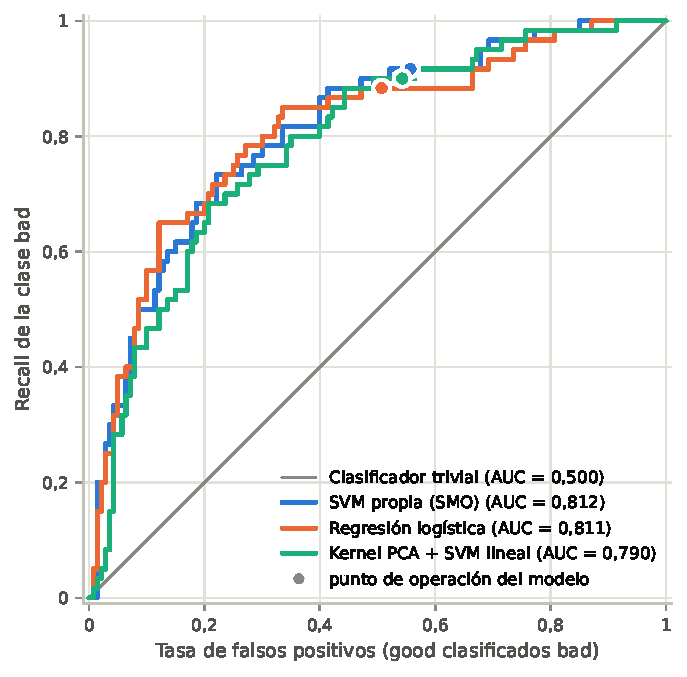
\includegraphics[width=0.6\textwidth]{roc_curves}
  \caption{Curvas ROC en test. El punto sobre cada curva es el punto de operación del modelo
  (el umbral con el que efectivamente clasifica).}
  \label{fig:roc}
\end{figure}

La tabla~\ref{tab:modelos} y la figura~\ref{fig:roc} resumen el resultado. La SVM propia
alcanza un AUC de \ResSvmAuc{} y un costo de \ResSvmCost{} (\ResSvmCostPer{} por
solicitante), contra \ResLogregCost{} de la regresión logística, \ResAlwaysBadCost{} de
rechazar a todos y \ResMajorityCost{} de aprobar a todos. Detecta el
\ResSvmRecall{} de los malos pagadores (\ResSvmTP{} de \ResNTestBad) a cambio de rechazar a
\ResSvmFP{} de los \ResNTestGood{} buenos.

Dos advertencias sobre la lectura de estos números. Primero, la diferencia entre la SVM y la
regresión logística (\ResSvmCost{} contra \ResLogregCost) es menor que el costo de un solo
falso negativo y no es estadísticamente significativa con \ResNTest{} casos de test: los
desvíos entre \emph{folds} de la tabla~\ref{tab:cv} son de ese orden. Lo que sí es robusto es
la distancia de ambos modelos a los clasificadores triviales. Segundo, el resultado coincide
con la literatura de \emph{credit scoring}, donde la regresión logística es un competidor
difícil de superar \cite{lessmann2015}.

\paragraph{Por qué la exactitud sola es engañosa.} El clasificador de clase mayoritaria
tiene la \emph{mejor} exactitud de la tabla (\ResMajorityAccuracy) y el \emph{peor} costo
(\ResMajorityCost): no detecta a ningún mal pagador. La SVM tiene una exactitud de apenas
\ResSvmAccuracy{} y el menor costo. Hay dos motivos. (i)~\emph{Desbalance}: con 70\,\% de
\good, la exactitud está dominada por la clase mayoritaria. (ii)~\emph{Asimetría de costos}:
la exactitud cuenta igual los dos errores, pero uno cuesta cinco veces más que el otro. Con
probabilidades calibradas, la regla que minimiza el costo esperado es rechazar cuando
$P(\bad\mid x) > c_{\mathrm{FP}}/(c_{\mathrm{FP}}+c_{\mathrm{FN}}) = 1/6$ \cite{elkan2001}:
un buen clasificador para este problema rechaza a propósito a muchos solicitantes que
probablemente pagarían, y por eso «se equivoca» más veces. Por eso se reportan el costo, el
\emph{recall} y la precisión de la clase \bad{} y el AUC (que mide la calidad del
ordenamiento con independencia del umbral).

\FloatBarrier
\subsection{Verificación de la implementación}

Con el mismo kernel e hiperparámetros, \code{sklearn.svm.SVC} y la SVM propia coinciden en
el \ResSkAgreement\,\% de las predicciones de test; la correlación entre sus funciones de
decisión es \ResSkCorr{} y la diferencia máxima, \ResSkMaxDiff{} (del orden de la tolerancia
KKT, \ResKktTol). Ambas encuentran \ResSkNSupport{} vectores de soporte. SMO convergió en
\ResSmoIter{} iteraciones (\ResFitSeconds\,s) con una brecha KKT final de \ResKktGap.

De los \ResNTrain{} puntos de entrenamiento, \ResNSupport{} (\ResSupportPct\,\%) son vectores
de soporte: \ResNFreeSupport{} libres (sobre el margen) y \ResNBoundSupport{} en la cota
$\alpha_i=C_i$ (dentro del margen o mal clasificados). Una proporción tan alta es esperable
cuando las clases se superponen mucho; la solución no es rala en este dataset.

\FloatBarrier
\subsection{Kernel PCA}

\begin{figure}[htbp]
  \centering
  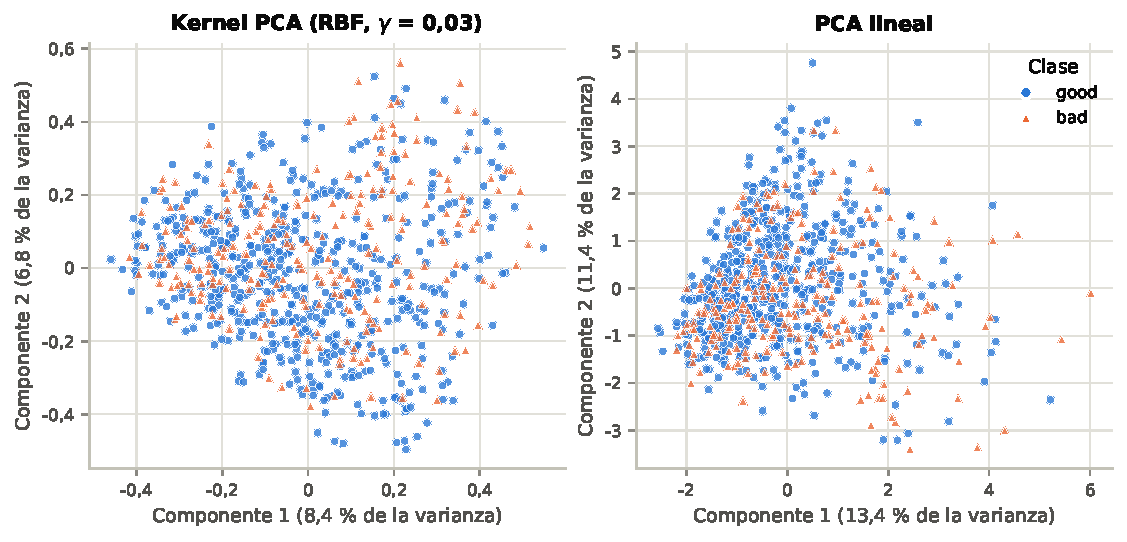
\includegraphics[width=\textwidth]{projection_kpca_vs_pca}
  \caption{Proyección del conjunto de entrenamiento sobre las dos primeras componentes
  principales: Kernel PCA con kernel RBF (izquierda) y PCA lineal (derecha).}
  \label{fig:proyeccion}
\end{figure}

\begin{figure}[htbp]
  \centering
  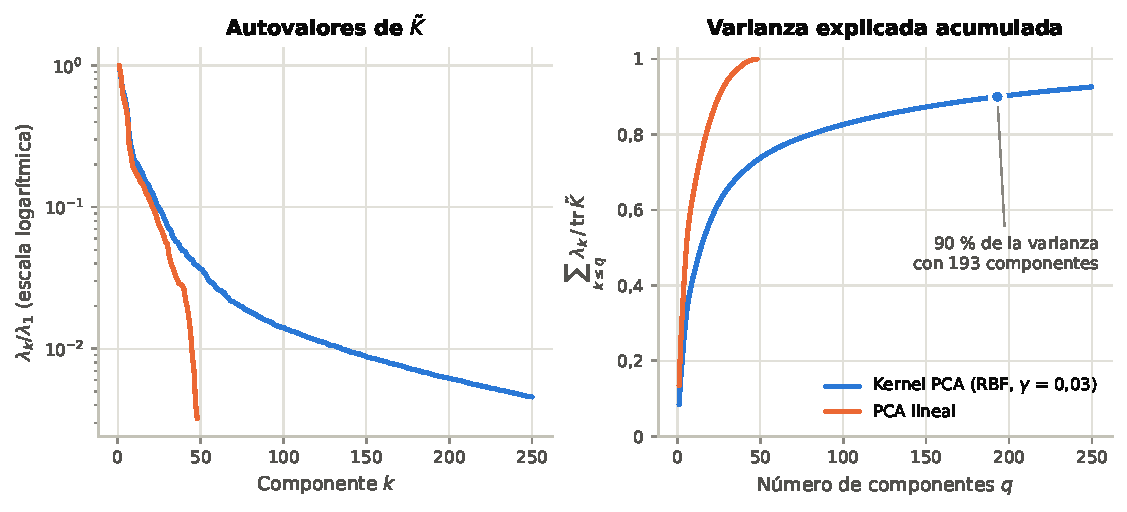
\includegraphics[width=\textwidth]{kpca_spectrum}
  \caption{Espectro de la matriz de Gram centrada $\Kc$ (izquierda, normalizado por
  $\lambda_1$) y varianza explicada acumulada (derecha) para los dos kernels de la
  figura~\ref{fig:proyeccion}.}
  \label{fig:espectro}
\end{figure}

Para las figuras se usó un $\gamma$ mayor que el elegido para clasificar, porque con el
$\gamma$ de la tabla~\ref{tab:cv} el kernel es casi lineal y Kernel PCA es indistinguible de
PCA. Las figuras~\ref{fig:proyeccion} y~\ref{fig:espectro} muestran tres cosas:
\begin{itemize}
  \item \textbf{Ninguna de las dos proyecciones separa las clases.} La información
        discriminante no está concentrada en las direcciones de mayor varianza: Kernel PCA
        no usa las etiquetas.
  \item \textbf{El kernel cambia la dimensión efectiva.} Con el kernel lineal, $\Kc$ tiene
        rango finito (a lo sumo el número de variables linealmente independientes) y el
        espectro se corta en seco. Con el kernel RBF el rango es $n-1$ y el espectro decae
        lentamente: hacen falta muchas más componentes para explicar la misma fracción de
        la varianza.
  \item \textbf{Las dos primeras componentes explican poca varianza} en ambos casos, de modo
        que un gráfico bidimensional es un resumen muy parcial de los datos.
\end{itemize}

\begin{figure}[htbp]
  \centering
  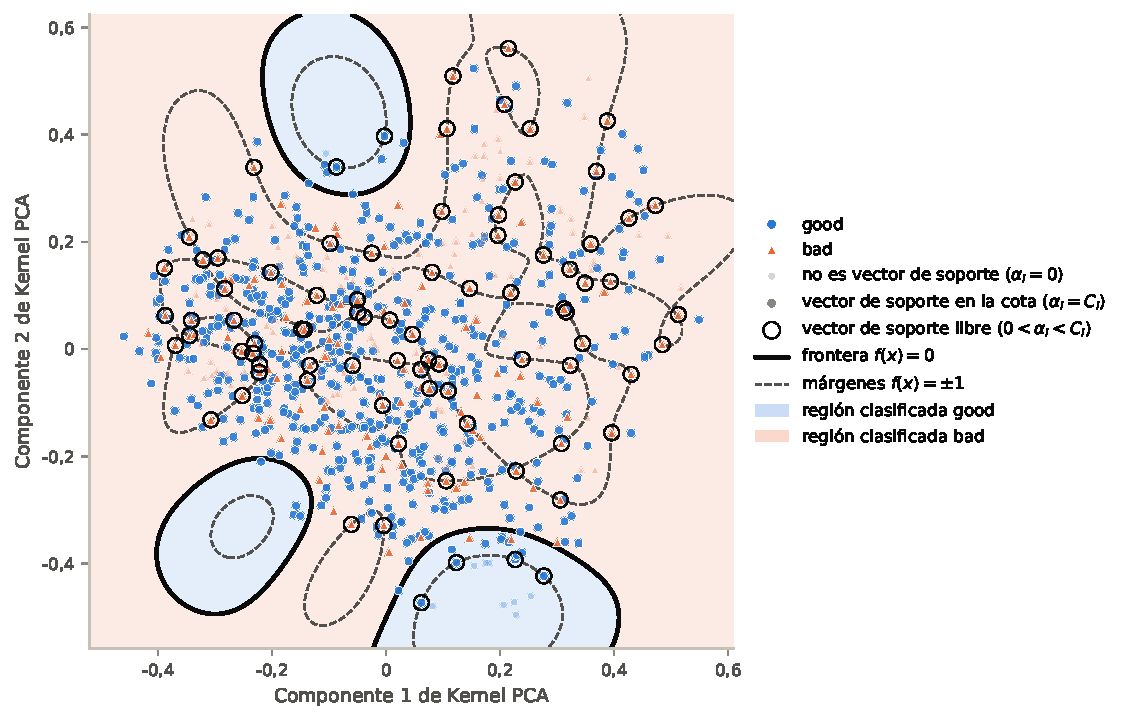
\includegraphics[width=0.95\textwidth]{svm_decision_boundary}
  \caption{SVM con kernel RBF entrenada sobre las dos primeras componentes de Kernel PCA
  (solo con fines ilustrativos), con los mismos pesos por clase que el modelo principal.}
  \label{fig:frontera}
\end{figure}

La figura~\ref{fig:frontera} ilustra la geometría de la SVM en ese plano. Se ven las
condiciones KKT de la ecuación~\eqref{eq:kkt-cases}: los vectores de soporte libres (con
anillo) caen sobre las curvas $f(x)=\pm1$; los puntos tenues, con $\alpha_i=0$, están del
lado correcto y fuera del margen; el resto son vectores de soporte en la cota. También se ve
el efecto del costo $5{:}1$: con solo dos componentes las clases se superponen tanto que la
SVM clasifica como \good{} únicamente las pocas regiones donde casi no hay \bad.

Como etapa del pipeline, Kernel PCA con 30 componentes seguido de una SVM lineal obtiene
un costo de \ResKpcaSvmCost{} y un AUC de \ResKpcaSvmAuc{} en test
(tabla~\ref{tab:modelos}): comparable a los otros modelos, sin mejorarlos.

\FloatBarrier
\subsection{Diagnóstico numérico}

La matriz de Gram de entrenamiento con el kernel elegido tiene autovalores entre
$\lambda_{\min}=\ResGramLambdaMin$ y $\lambda_{\max}=\ResGramLambdaMax$: es definida positiva
(rango numérico \ResGramRank) pero está mal condicionada, con
$\kappa_2(K)=\ResGramCond$. El \emph{jitter} $\varepsilon=\ResGramJitter$ que se suma a la
diagonal deja $\kappa_2(K+\varepsilon I)=\ResGramCondJitter$: aquí casi no cambia nada,
porque $\varepsilon\ll\lambda_{\min}$; su función es de resguardo para el caso en que haya
puntos repetidos y $K$ sea singular (sección~\ref{sec:estabilidad}). La matriz centrada
$\Kc$ tiene rango numérico \ResCenteredRank{} $=n-1$, como predice la teoría
(ecuación~\eqref{eq:centered-zero-sums}), y número de condición efectivo \ResCenteredCond.
Ni SMO ni Kernel PCA invierten $K$, de modo que este mal condicionamiento no degrada los
resultados; sí importaría en las extensiones que resuelven sistemas lineales con $K$
(sección~\ref{sec:roadmap}).

\FloatBarrier
\subsection{Análisis de variables sensibles}\label{sec:sensibles}

El dataset incluye tres atributos sensibles: \code{personal\_status} (estado civil y sexo),
\code{age} (edad) y \code{foreign\_worker} (trabajador extranjero). Se entrenó la SVM con y
sin esos atributos (repitiendo la validación cruzada en cada caso) y se midieron, en test,
la tasa de aprobación, el \emph{recall} de \bad{} y la tasa de falsos positivos (TFP: buenos
pagadores rechazados) por subgrupo. Los grupos son: sexo, leído del prefijo de
\code{personal\_status}; edad $\le\ResAgeThreshold$ años frente a mayores, un corte usual en
la literatura sobre este dataset \cite{kamiran2012}; y \code{foreign\_worker}.

\begin{table}[H]
  \centering
  \small
  \begin{tabular}{lrrrrrrr}
\toprule
Modelo & AUC & Recall \emph{bad} & Precisión \emph{bad} & Costo & $\Delta$ sexo & $\Delta$ edad & $\Delta$ extranjero \\
\midrule
Con atributos sensibles & \num{0.812} & \num{0.917} & \num{0.414} & \num{103} & \num{0.128} & \num{0.138} & \num{0.342} \\
Sin atributos sensibles & \num{0.803} & \num{0.900} & \num{0.397} & \num{112} & \num{0.036} & \num{0.090} & \num{0.014} \\
\bottomrule
\end{tabular}

  \caption{SVM con y sin atributos sensibles (test). \emph{Recall} y precisión de la clase
  \bad. $\Delta$: diferencia máxima de tasa de aprobación entre los grupos de cada atributo.}
  \label{tab:sensibles}
\end{table}

\begin{table}[H]
  \centering
  \small
  \begin{tabular}{llrrrrrrrr}
\toprule
& & & & \multicolumn{3}{c}{Con atributos sensibles} & \multicolumn{3}{c}{Sin atributos sensibles} \\
\cmidrule(lr){5-7} \cmidrule(lr){8-10}
Atributo & Grupo & $n$ & $n_{\text{bad}}$ & Aprob. & Recall & TFP & Aprob. & Recall & TFP \\
\midrule
Sexo & female & \num{61} & \num{20} & \num{0.25} & \num{0.95} & \num{0.66} & \num{0.30} & \num{0.95} & \num{0.59} \\
Sexo & male & \num{139} & \num{40} & \num{0.37} & \num{0.90} & \num{0.52} & \num{0.33} & \num{0.88} & \num{0.59} \\
\midrule
Edad & $\leq$25 & \num{44} & \num{20} & \num{0.23} & \num{0.95} & \num{0.62} & \num{0.25} & \num{0.90} & \num{0.62} \\
Edad & $>$25 & \num{156} & \num{40} & \num{0.37} & \num{0.90} & \num{0.54} & \num{0.34} & \num{0.90} & \num{0.58} \\
\midrule
Trabajador extranjero & no & \num{6} & \num{1} & \num{0.67} & \num{1.00} & \num{0.20} & \num{0.33} & \num{1.00} & \num{0.60} \\
Trabajador extranjero & yes & \num{194} & \num{59} & \num{0.32} & \num{0.92} & \num{0.57} & \num{0.32} & \num{0.90} & \num{0.59} \\
\bottomrule
\end{tabular}

  \caption{Métricas por subgrupo en test. Aprob.: tasa de aprobación (fracción predicha
  \good); Recall: fracción de los \bad{} del grupo detectados; TFP: fracción de los \good{}
  del grupo rechazados. $n_{\text{bad}}$ pequeños hacen poco fiables las tasas.}
  \label{tab:subgrupos}
\end{table}

\paragraph{Lectura.} Con los atributos sensibles, el modelo aprueba menos a las mujeres y a
los menores de \ResAgeThreshold{} años (brechas de aprobación de \ResSensGapSex{} y
\ResSensGapAge), y les rechaza una fracción mayor de buenos pagadores. Al quitar los
atributos, la brecha por sexo baja a \ResNoSensGapSex{} y la de edad a \ResNoSensGapAge, y
las tasas de falsos positivos se acercan entre grupos. El precio es una pérdida moderada de
desempeño: el costo pasa de \ResSensCost{} a \ResNoSensCost{} y el AUC de \ResSensAuc{} a
\ResNoSensAuc.

\paragraph{Implicancias y cautelas.}
\begin{itemize}
  \item \textbf{Quitar el atributo no quita la información.} Otros atributos (vivienda,
        empleo, antigüedad, monto) están correlacionados con la edad y el sexo y actúan como
        variables sustitutas; la «equidad por desconocimiento» no garantiza la paridad entre
        grupos \cite{barocas2023}. La brecha residual por edad lo muestra.
  \item \textbf{Los criterios de equidad compiten entre sí.} Igualar tasas de aprobación
        (paridad demográfica) e igualar tasas de error por grupo (igualdad de oportunidades,
        \cite{hardt2016}) son objetivos distintos y, cuando las tasas base difieren entre
        grupos, en general incompatibles. Aquí difieren (columna $n_{\text{bad}}/n$ de la
        tabla~\ref{tab:subgrupos}).
  \item \textbf{Muestras chicas.} El grupo \code{foreign\_worker = no} tiene muy pocos casos
        en test; sus tasas, y la brecha correspondiente, no son estimaciones fiables. En
        general, con \ResNTest{} casos todas las diferencias por subgrupo tienen intervalos
        de confianza amplios.
  \item \textbf{Calidad del dato.} Grömping \cite{gromping2019} documenta errores de
        codificación en la versión Statlog; entre ellos, que \code{personal\_status} no
        permitiría recuperar el sexo de manera fiable y que las etiquetas de
        \code{foreign\_worker} estarían invertidas. Estas tablas deben leerse como un
        ejercicio metodológico, no como evidencia sobre grupos reales.
  \item \textbf{Marco normativo.} En muchas jurisdicciones el uso de atributos como el sexo
        o la nacionalidad en decisiones de crédito está restringido o prohibido. Por eso el
        pipeline permite excluirlos por configuración (\code{data.exclude\_sensitive: true})
        sin tocar código, y las métricas por subgrupo se calculan siempre a partir de los
        datos crudos, también para el modelo que no los usa.
\end{itemize}

\FloatBarrier
% =============================================================================
\section{Limitaciones}\label{sec:limitaciones}
% =============================================================================

\begin{itemize}
  \item \textbf{Tamaño de muestra.} Con \ResNSamples{} observaciones y un único conjunto de
        test de \ResNTest{}, las diferencias entre modelos buenos están dentro del ruido. No
        se hizo validación cruzada anidada: el costo de validación del mejor punto de la
        grilla es una estimación optimista.
  \item \textbf{Escalabilidad.} La matriz de Gram ocupa $O(n^2)$ memoria, cada iteración de
        SMO cuesta $O(n)$ y Kernel PCA cuesta $O(n^3)$. Sin caché de kernel, \emph{shrinking}
        ni selección de segundo orden \cite{fan2005}, la implementación es adecuada hasta
        $n\sim10^4$, no más.
  \item \textbf{Convergencia de SMO.} La regla de primer orden puede necesitar muchas
        iteraciones cuando $C$ es grande o el problema tiene pocas dimensiones y clases muy
        superpuestas; el código avisa si alcanza \code{max\_iter} sin cumplir la tolerancia.
  \item \textbf{Sin probabilidades.} La SVM entrega un puntaje sin calibrar. El costo
        asimétrico se incorpora con pesos por clase, que es un sustituto convexo del costo
        (ecuación~\eqref{eq:weighted-hinge-bound}), no su minimización directa; no se ajusta
        el umbral de decisión.
  \item \textbf{Variables categóricas.} La codificación \emph{one-hot} con distancia
        euclídea trata todas las categorías como equidistantes e ignora el orden de las
        ordinales; los atributos numéricos asimétricos (monto, duración) no se transforman.
  \item \textbf{Kernel PCA no es supervisado.} Sus componentes maximizan varianza, no
        separación de clases; como reducción de dimensión previa puede descartar señal.
  \item \textbf{El dataset.} Es antiguo, pequeño, contiene solo solicitudes \emph{aprobadas}
        (sesgo de selección: no se observa el comportamiento de los rechazados) y tiene los
        problemas de codificación mencionados en la sección~\ref{sec:sensibles}. Los
        resultados no son extrapolables a una cartera actual.
  \item \textbf{Análisis de equidad descriptivo.} Se miden brechas, no se corrigen; los
        subgrupos son pequeños y los atributos sensibles, de calidad dudosa.
\end{itemize}

% =============================================================================
\section{Roadmap de extensiones}\label{sec:roadmap}
% =============================================================================

Ordenadas de menor a mayor dificultad. Para cada una se indica qué partes del código toca.

\begin{enumerate}
  \item \textbf{Kernels para variables categóricas} (dificultad baja). En lugar de
        \emph{one-hot} + RBF, usar un kernel de coincidencias
        $k(x,y)=\sum_j \ones[x_j=y_j]$ o su versión exponencial sobre la distancia de
        Hamming, y combinarlo con un RBF sobre las variables numéricas mediante suma o
        producto. Solo requiere una subclase de \code{Kernel} registrada y que el
        preprocesador entregue los bloques por separado; la validez del kernel combinado
        está garantizada por la sección~\ref{sec:schur}.
  \item \textbf{Calibración de probabilidades (Platt scaling)} (baja). Ajustar una sigmoide
        $P(\bad\mid x)=1/(1+e^{Af(x)+B})$ a los puntajes de validación cruzada
        \cite{platt1999}. Con probabilidades calibradas se puede aplicar el umbral óptimo
        $1/6$ de la matriz de costos y comparar con el enfoque de pesos por clase. Toca
        \code{pipeline} (una etapa más) y \code{evaluation} (curvas de calibración).
  \item \textbf{Aproximación de Nyström y \emph{features} aleatorias de Fourier} (media).
        Para $n$ grande, reemplazar $K$ por una aproximación de rango $m\ll n$:
        Nyström usa $K\approx K_{nm}K_{mm}^{-1}K_{mn}$ con $m$ puntos de referencia
        \cite{williams2001}; las \emph{features} de Fourier aproximan un kernel invariante
        por traslaciones con $z(x)=\sqrt{2/D}\cos(Wx+b)$ \cite{rahimi2007}. En ambos casos
        se obtiene un mapa de características explícito y el problema pasa a ser lineal.
        Nyström invierte $K_{mm}$: ahí el \emph{jitter} y el número de condición de la
        sección~\ref{sec:estabilidad} dejan de ser un resguardo y pasan a ser necesarios.
  \item \textbf{Aprendizaje de múltiples kernels} (media--alta). Aprender los pesos
        $\mu_m\ge0$ de una combinación $k=\sum_m\mu_m k_m$ (por ejemplo, un kernel por grupo
        de atributos) junto con la SVM \cite{lanckriet2004,rakotomamonjy2008}. La
        composición de kernels ya existe; falta el lazo externo de optimización sobre
        $\mu$, que alterna con SMO.
  \item \textbf{Datasets de crédito más grandes} (alta). Carteras con $10^5$--$10^6$
        solicitudes exigen las aproximaciones anteriores, un optimizador lineal (descenso
        por coordenadas en el dual o gradiente estocástico), validación temporal en lugar de
        aleatoria, tratamiento de faltantes e inferencia sobre rechazados. Es un cambio de
        escala que afecta a \code{data}, \code{svm} y \code{tuning}.
\end{enumerate}

\clearpage
% =============================================================================
\appendix
\section{Apéndice matemático formal}\label{sec:apendice}
% =============================================================================

\paragraph{Convenciones.} Los espacios vectoriales son reales salvo indicación contraria.
$A^{\dg}$ denota la traspuesta conjugada de $A$, que para matrices y vectores reales es
la traspuesta: $u^{\dg}v$ es el producto interno usual de $\R^n$ y $\ones$ es el vector de
unos, de modo que $\ones^{\dg}\ones=n$. $I$ es la identidad, $e_i$ el $i$-ésimo vector
canónico, $A\circ B$ el producto de Hadamard (entrada a entrada) y $A\succeq0$ indica que $A$
es simétrica semidefinida positiva. Las ecuaciones de este apéndice son las que citan los
comentarios del código, en la forma «Ec.~(A.$n$)~[\code{eq:etiqueta}]».

% -----------------------------------------------------------------------------
\subsection{Kernels definidos positivos y espacios de Hilbert con núcleo reproductor}
\label{sec:rkhs}

\begin{definicion}[Kernel definido positivo]
Sea $\X$ un conjunto no vacío. Una función $k\colon\X\times\X\to\R$ es un \emph{kernel
definido positivo} si es simétrica, $k(x,y)=k(y,x)$, y para todo $n\in\N$, todos
$x_1,\dots,x_n\in\X$ y todo $c\in\R^n$,
\begin{equation}\label{eq:pd-kernel}
  \sum_{i=1}^n\sum_{j=1}^n c_i\,c_j\,k(x_i,x_j) \;=\; c^{\dg}Kc \;\ge\; 0,
  \qquad K=\bigl[k(x_i,x_j)\bigr]_{i,j=1}^n .
\end{equation}
La matriz $K$ es la \emph{matriz de Gram} de $x_1,\dots,x_n$.
\end{definicion}

En la literatura de kernels «definido positivo» corresponde a lo que para matrices se llama
\emph{semidefinido} positivo: \eqref{eq:pd-kernel} dice exactamente que toda matriz de Gram
es simétrica semidefinida positiva.

\begin{proposicion}[Todo mapa de características define un kernel]\label{prop:feature}
Si $\Hk$ es un espacio de Hilbert y $\varphi\colon\X\to\Hk$ es cualquier función, entonces
$k(x,y)=\inner{\varphi(x)}{\varphi(y)}_{\Hk}$ es un kernel definido positivo.
\end{proposicion}
\begin{proof}
La simetría es la del producto interno real. Por bilinealidad,
\begin{equation}\label{eq:feature-kernel}
  c^{\dg}Kc=\sum_{i,j}c_i c_j\inner{\varphi(x_i)}{\varphi(x_j)}_{\Hk}
  =\Bigl\lVert\sum_{i=1}^n c_i\,\varphi(x_i)\Bigr\rVert_{\Hk}^2\ \ge\ 0. \qedhere
\end{equation}
\end{proof}

\begin{definicion}[RKHS]
Un espacio de Hilbert $\Hk$ cuyos elementos son funciones $f\colon\X\to\R$ (con las
operaciones puntuales) es un \emph{espacio de Hilbert con núcleo reproductor} (RKHS) si para
cada $x\in\X$ el funcional de evaluación $\delta_x\colon f\mapsto f(x)$ es continuo.
\end{definicion}

\begin{proposicion}[Núcleo reproductor]\label{prop:nucleo}
Sea $\Hk$ un RKHS sobre $\X$. Existe una única función $k\colon\X\times\X\to\R$ tal que
$k(\cdot,x)\in\Hk$ para todo $x\in\X$ y se cumple la \emph{propiedad reproductora}
\begin{equation}\label{eq:reproducing}
  f(x)=\inner{f}{k(\cdot,x)}_{\Hk}\qquad\text{para todo } f\in\Hk,\ x\in\X .
\end{equation}
Además $k$ es un kernel definido positivo, y
\begin{align}
  k(x,y) &= \inner{k(\cdot,y)}{k(\cdot,x)}_{\Hk}, \label{eq:kernel-from-rk}\\
  \abs{f(x)} &\le \norm{f}_{\Hk}\sqrt{k(x,x)}. \label{eq:eval-bound}
\end{align}
\end{proposicion}
\begin{proof}
Como $\delta_x$ es lineal y continuo, el teorema de representación de Riesz da un único
$k_x\in\Hk$ con $f(x)=\inner{f}{k_x}$ para todo $f$. Definiendo $k(y,x)=k_x(y)$ se obtiene
\eqref{eq:reproducing}. Aplicando \eqref{eq:reproducing} a $f=k(\cdot,y)$ resulta
\eqref{eq:kernel-from-rk}, que muestra que $k$ es simétrico y que tiene la forma de la
proposición~\ref{prop:feature} con $\varphi(x)=k(\cdot,x)$; luego es definido positivo.
La cota \eqref{eq:eval-bound} es la desigualdad de Cauchy--Schwarz en \eqref{eq:reproducing},
con $\norm{k(\cdot,x)}^2=k(x,x)$. Unicidad: si $k'$ también reproduce, entonces
$\inner{f}{k(\cdot,x)-k'(\cdot,x)}=0$ para todo $f$, y $k(\cdot,x)=k'(\cdot,x)$.
\end{proof}

\begin{observacion}
La cota \eqref{eq:eval-bound} es la diferencia esencial con $L^2$: en un RKHS la
convergencia en norma implica convergencia puntual. El mapa canónico
$\varphi(x)=k(\cdot,x)$ realiza el truco del kernel~\eqref{eq:truco}:
$k(x,y)=\inner{\varphi(x)}{\varphi(y)}_{\Hk}$.
\end{observacion}

% -----------------------------------------------------------------------------
\subsection{Teorema de Moore--Aronszajn}

La proposición~\ref{prop:nucleo} asocia a cada RKHS un kernel definido positivo. El teorema
siguiente es el recíproco: el kernel determina el espacio.

\begin{teorema}[Moore--Aronszajn \cite{aronszajn1950}]\label{teo:moore}
Sea $k$ un kernel definido positivo sobre $\X$. Existe un único espacio de Hilbert $\Hk_k$ de
funciones sobre $\X$ cuyo núcleo reproductor es $k$. Además,
$\Hk_0=\gen\{k(\cdot,x):x\in\X\}$ es denso en $\Hk_k$.
\end{teorema}
\begin{proof}
\emph{Paso 1: producto interno en $\Hk_0$.} Para $f=\sum_{i=1}^m a_i\,k(\cdot,x_i)$ y
$g=\sum_{j=1}^r b_j\,k(\cdot,y_j)$ en $\Hk_0$ se define
\begin{equation}\label{eq:pre-rkhs-inner}
  \inner{f}{g}_0=\sum_{i=1}^m\sum_{j=1}^r a_i\,b_j\,k(x_i,y_j)
  =\sum_{j=1}^r b_j\,f(y_j)=\sum_{i=1}^m a_i\,g(x_i).
\end{equation}
Las dos últimas expresiones muestran que el valor depende solo de $f$ y $g$ como funciones,
no de las representaciones elegidas. La forma es bilineal y simétrica, y
$\inner{f}{f}_0=a^{\dg}Ka\ge0$ por \eqref{eq:pd-kernel}. Tomando $g=k(\cdot,x)$ se obtiene
$\inner{f}{k(\cdot,x)}_0=f(x)$. Una forma bilineal simétrica semidefinida positiva cumple la
desigualdad de Cauchy--Schwarz, de modo que
\begin{equation}\label{eq:pre-rkhs-bound}
  \abs{f(x)}^2=\inner{f}{k(\cdot,x)}_0^2\le\inner{f}{f}_0\;k(x,x).
\end{equation}
Así, $\inner{f}{f}_0=0$ implica $f\equiv0$: $\inner{\cdot}{\cdot}_0$ es un producto interno,
con norma $\norm{\cdot}_0$.

\emph{Paso 2: completación por funciones.} Si $(f_n)$ es de Cauchy en $\Hk_0$, por
\eqref{eq:pre-rkhs-bound} aplicada a $f_n-f_m$ la sucesión $(f_n(x))$ es de Cauchy en $\R$
para cada $x$; sea $f(x)=\lim_n f_n(x)$. Se define $\Hk_k$ como el conjunto de las funciones
$f$ que se obtienen así; contiene a $\Hk_0$. El punto delicado es el siguiente.

\emph{Lema.} Si $(f_n)$ es de Cauchy en $\Hk_0$ y $f_n(x)\to0$ para todo $x$, entonces
$\norm{f_n}_0\to0$. En efecto, sea $B$ una cota de $\norm{f_n}_0$. Dado $\varepsilon>0$, sea
$N$ tal que $\norm{f_n-f_N}_0\le\varepsilon/B$ si $n\ge N$, y escribamos
$f_N=\sum_{i=1}^m a_i\,k(\cdot,x_i)$. Para $n\ge N$,
\[
  \norm{f_n}_0^2=\inner{f_n-f_N}{f_n}_0+\inner{f_N}{f_n}_0
  \le\varepsilon+\sum_{i=1}^m a_i\,f_n(x_i),
\]
y la última suma tiende a $0$. Luego $\limsup_n\norm{f_n}_0^2\le\varepsilon$ para todo
$\varepsilon>0$.

Para $f,g\in\Hk_k$ con sucesiones aproximantes $(f_n)$, $(g_n)$ se define
$\inner{f}{g}=\lim_n\inner{f_n}{g_n}_0$. El límite existe, porque
$\abs{\inner{f_n}{g_n}_0-\inner{f_m}{g_m}_0}\le\norm{f_n-f_m}_0\norm{g_n}_0
+\norm{f_m}_0\norm{g_n-g_m}_0$, y por el lema no depende de las sucesiones elegidas: si
$(f_n')$ tiene el mismo límite puntual, $(f_n-f_n')$ es de Cauchy con límite puntual nulo y
$\norm{f_n-f_n'}_0\to0$. Es un producto interno que extiende $\inner{\cdot}{\cdot}_0$: si
$\inner{f}{f}=0$ entonces $\norm{f_n}_0\to0$ y, por \eqref{eq:pre-rkhs-bound},
$f(x)=\lim_n f_n(x)=0$.

\emph{Paso 3: $\Hk_k$ es un RKHS con núcleo $k$.} Por construcción,
$\norm{f-f_n}=\lim_m\norm{f_m-f_n}_0\to0$: $\Hk_0$ es denso en $\Hk_k$ y toda sucesión de
Cauchy de $\Hk_0$ converge en $\Hk_k$. Un espacio métrico con un subconjunto denso cuyas
sucesiones de Cauchy convergen en el espacio es completo; luego $\Hk_k$ es de Hilbert. Para
$f\in\Hk_k$ con $f_n\to f$,
$\inner{f}{k(\cdot,x)}=\lim_n\inner{f_n}{k(\cdot,x)}_0=\lim_n f_n(x)=f(x)$:
se cumple \eqref{eq:reproducing}, y por lo tanto la evaluación es continua.

\emph{Paso 4: unicidad.} Sea $\mathcal G$ otro RKHS con núcleo $k$. Entonces
$\Hk_0\subset\mathcal G$ y, por \eqref{eq:kernel-from-rk}, los productos internos de
$\mathcal G$ y $\Hk_k$ coinciden en $\Hk_0$. Además $\Hk_0$ es denso en $\mathcal G$: si
$g\in\mathcal G$ es ortogonal a todo $k(\cdot,x)$, entonces $g(x)=\inner{g}{k(\cdot,x)}=0$.
Cada $g\in\mathcal G$ es límite en norma, y por \eqref{eq:eval-bound} límite puntual, de una
sucesión de Cauchy de $\Hk_0$; es decir, es un elemento de $\Hk_k$ con la misma norma. El
argumento simétrico da la otra inclusión.
\end{proof}

\begin{ejemplo}
Para el kernel lineal $k(x,y)=x^{\dg}y$ en $\R^d$, $\Hk_k=\{x\mapsto w^{\dg}x: w\in\R^d\}$
con $\norm{f}_{\Hk_k}=\norm{w}$: el RKHS son las funciones lineales. Para el kernel gaussiano,
$\Hk_k$ tiene dimensión infinita y está formado por funciones analíticas
\cite[sección 4.4]{steinwart2008}. Tratamientos completos de la teoría:
\cite{berlinet2004,paulsen2016}.
\end{ejemplo}

% -----------------------------------------------------------------------------
\subsection{Teorema de Mercer}

Moore--Aronszajn construye el espacio de características de manera abstracta. El teorema de
Mercer lo describe de manera espectral, bajo hipótesis topológicas.

\begin{teorema}[Mercer \cite{mercer1909}; ver {\cite[teorema 4.49]{steinwart2008}}]
\label{teo:mercer}
Sean $\X$ un espacio métrico compacto, $\mu$ una medida de Borel finita sobre $\X$ con
soporte igual a $\X$, y $k\colon\X\times\X\to\R$ un kernel definido positivo y continuo.
Entonces el operador integral
\begin{equation}\label{eq:mercer-operator}
  (T_kf)(x)=\int_{\X}k(x,y)\,f(y)\,d\mu(y),\qquad f\in L^2(\X,\mu),
\end{equation}
es compacto, autoadjunto ($T_k^{\dg}=T_k$) y positivo. Existe una familia ortonormal a lo
sumo numerable $(e_j)_{j\in J}$ de $L^2(\X,\mu)$, formada por autofunciones continuas de
$T_k$ con autovalores $\lambda_j>0$ (con $\lambda_j\to0$ si $J$ es infinito), tal que
\begin{equation}\label{eq:mercer-expansion}
  k(x,y)=\sum_{j\in J}\lambda_j\,e_j(x)\,e_j(y)\qquad\text{para todo }x,y\in\X,
\end{equation}
con convergencia absoluta y uniforme en $\X\times\X$.
\end{teorema}

No se incluye la demostración, que requiere el teorema espectral para operadores compactos
autoadjuntos y el teorema de Dini; puede verse en
\cite[sección 4.5]{steinwart2008} o \cite{cuckersmale2002}. Sobre las hipótesis:
\begin{itemize}
  \item La \emph{compacidad} de $\X$ y la \emph{continuidad} de $k$ dan la compacidad de
        $T_k$ y la convergencia uniforme. En dominios no compactos (por ejemplo, el kernel
        gaussiano en todo $\R^d$) el enunciado no se aplica tal cual; hay generalizaciones
        en \cite{steinwartscovel2012}.
  \item La \emph{simetría} da $T_k^{\dg}=T_k$, y la \emph{positividad}
        \eqref{eq:pd-kernel} equivale a $\inner{T_kf}{f}_{L^2}\ge0$, es decir, a
        $\lambda_j\ge0$.
  \item El \emph{soporte total} de $\mu$ garantiza que \eqref{eq:mercer-expansion} valga en
        todo punto y no solo en casi todo punto.
\end{itemize}
Una consecuencia es un mapa de características explícito hacia $\ell^2$:
$\varphi(x)=\bigl(\sqrt{\lambda_j}\,e_j(x)\bigr)_{j\in J}$ cumple
$k(x,y)=\inner{\varphi(x)}{\varphi(y)}_{\ell^2}$.

\paragraph{Relación con la matriz de Gram.} Sea $\mu_n=\frac1n\sum_{i=1}^n\delta_{x_i}$ la
medida empírica de la muestra, sobre el conjunto finito (compacto) $\{x_1,\dots,x_n\}$.
Entonces $L^2(\mu_n)\cong\R^n$ con producto interno $\frac1n f^{\dg}g$, y el operador
\eqref{eq:mercer-operator} es
\begin{equation}\label{eq:empirical-operator}
  (T_kf)(x_i)=\frac1n\sum_{j=1}^nK_{ij}\,f(x_j),\qquad\text{es decir,}\qquad T_k=\tfrac1nK .
\end{equation}
El teorema de Mercer para $\mu_n$ es el teorema espectral para la matriz simétrica $K$
(teorema~\ref{teo:espectral}):
\begin{equation}\label{eq:gram-spectral}
  K=\sum_{j=1}^n\lambda_j\,u_ju_j^{\dg},\qquad
  K_{il}=\sum_{j=1}^n\lambda_j\,u_{j,i}\,u_{j,l},
\end{equation}
con $e_j=\sqrt n\,u_j$ (ortonormales en $L^2(\mu_n)$) y autovalores $\lambda_j/n$ de $T_k$.
Los autovalores de $K/n$ son, entonces, la versión muestral de los autovalores de Mercer, y
convergen a ellos cuando $n\to\infty$ bajo condiciones adecuadas \cite{koltchinskii2000}.
Eso es lo que calcula Kernel PCA (tras centrar) y lo que muestra la
figura~\ref{fig:espectro}.

% -----------------------------------------------------------------------------
\subsection{Teorema del representante}

\begin{teorema}[Kimeldorf--Wahba \cite{kimeldorf1971}; Schölkopf--Herbrich--Smola
\cite{scholkopf2001}]\label{teo:representante}
Sean $\Hk$ un RKHS sobre $\X$ con núcleo $k$, $x_1,\dots,x_n\in\X$,
$L\colon\R^n\to\R\cup\{+\infty\}$ una función arbitraria y $\Omega\colon[0,\infty)\to\R$
estrictamente creciente. Todo minimizador $f^\star$ de
\begin{equation}\label{eq:representer-objective}
  J(f)=L\bigl(f(x_1),\dots,f(x_n)\bigr)+\Omega\bigl(\norm{f}_{\Hk}\bigr),\qquad f\in\Hk,
\end{equation}
admite una representación
\begin{equation}\label{eq:representer-form}
  f^\star=\sum_{i=1}^n\alpha_i\,k(\cdot,x_i),\qquad\alpha\in\R^n .
\end{equation}
\end{teorema}
\begin{proof}
Sea $V=\gen\{k(\cdot,x_1),\dots,k(\cdot,x_n)\}$. Como $V$ tiene dimensión finita es cerrado,
y $\Hk=V\oplus V^{\perp}$: todo $f\in\Hk$ se escribe $f=f_V+f_\perp$ con $f_V\in V$ y
$f_\perp\perp V$. Por la propiedad reproductora \eqref{eq:reproducing},
\begin{equation}\label{eq:representer-eval}
  f(x_i)=\inner{f_V+f_\perp}{k(\cdot,x_i)}_{\Hk}=\inner{f_V}{k(\cdot,x_i)}_{\Hk}=f_V(x_i),
  \qquad i=1,\dots,n,
\end{equation}
de modo que el término $L$ toma el mismo valor en $f$ y en $f_V$. Por el teorema de Pitágoras,
\begin{equation}\label{eq:representer-norm}
  \norm{f}_{\Hk}^2=\norm{f_V}_{\Hk}^2+\norm{f_\perp}_{\Hk}^2\ \ge\ \norm{f_V}_{\Hk}^2,
\end{equation}
con desigualdad estricta si $f_\perp\ne0$. Como $\Omega$ es estrictamente creciente,
$J(f_V)<J(f)$ siempre que $f_\perp\ne0$. Luego un minimizador cumple $f_\perp=0$, es decir,
pertenece a $V$.
\end{proof}

\begin{corolario}[Reducción a dimensión finita]\label{cor:finito}
Para $f$ de la forma \eqref{eq:representer-form},
\begin{equation}\label{eq:rkhs-norm-gram}
  f(x_j)=(K\alpha)_j,\qquad\norm{f}_{\Hk}^2=\alpha^{\dg}K\alpha ,
\end{equation}
y minimizar $J$ sobre $\Hk$ equivale a minimizar
$L(K\alpha)+\Omega\bigl(\sqrt{\alpha^{\dg}K\alpha}\bigr)$ sobre $\alpha\in\R^n$.
\end{corolario}

\begin{observacion}[Término de sesgo]\label{obs:sesgo}
La SVM usa funciones $f=h+b$ con $h\in\Hk$ y un sesgo $b\in\R$ que no se penaliza. Para cada
$b$ fijo el teorema se aplica a $h$ con $L_b(t)=L(t+b\,\ones)$: en el óptimo
$h=\sum_i\alpha_i\,k(\cdot,x_i)$. Si $\Omega$ es solo no decreciente, el mismo argumento
muestra que, si hay un minimizador, hay uno de la forma \eqref{eq:representer-form}.
\end{observacion}

% -----------------------------------------------------------------------------
\subsection{Sumas y productos de kernels: el producto de Schur}\label{sec:schur}

\begin{proposicion}\label{prop:suma}
Si $k_1,k_2$ son kernels definidos positivos sobre $\X$ y $a\ge0$, entonces $a\,k_1$ y
$k_1+k_2$ también lo son. El límite puntual de kernels definidos positivos es definido
positivo.
\end{proposicion}
\begin{proof}
Con $K_1,K_2$ las matrices de Gram de una misma muestra,
\begin{equation}\label{eq:sum-kernel}
  c^{\dg}(a\,K_1+K_2)\,c=a\,c^{\dg}K_1c+c^{\dg}K_2c\ \ge\ 0 .
\end{equation}
Para el límite puntual, \eqref{eq:pd-kernel} es un límite de números no negativos.
\end{proof}

\begin{teorema}[Producto de Schur \cite{schur1911}]\label{teo:schur}
Si $A,B\in\R^{n\times n}$ son simétricas semidefinidas positivas, también lo es su producto
de Hadamard $A\circ B$, $(A\circ B)_{ij}=A_{ij}B_{ij}$.
\end{teorema}
\begin{proof}
Por el teorema espectral (teorema~\ref{teo:espectral}),
$B=\sum_{r=1}^n\mu_r\,v_rv_r^{\dg}$ con $\mu_r\ge0$. Para $c\in\R^n$,
\begin{equation}\label{eq:schur}
  c^{\dg}(A\circ B)\,c=\sum_{i,j}c_ic_jA_{ij}\sum_{r}\mu_r\,v_{r,i}v_{r,j}
  =\sum_{r=1}^n\mu_r\,(c\circ v_r)^{\dg}A\,(c\circ v_r)\ \ge\ 0,
\end{equation}
porque cada sumando es $\mu_r\ge0$ por una forma cuadrática de $A\succeq0$.
\end{proof}

\begin{corolario}\label{cor:producto}
Sean $k,k_1,k_2$ kernels definidos positivos sobre $\X$. Entonces también lo son:
\begin{enumerate}[label=(\alph*)]
  \item el producto $k_1k_2$ (su matriz de Gram es $K_1\circ K_2$);
  \item $p(k)$ para todo polinomio $p$ con coeficientes no negativos, y $\exp(k)$ (límite
        puntual de tales polinomios);
  \item $g(x)\,k(x,y)\,g(y)$ para toda $g\colon\X\to\R$, pues
        $c^{\dg}K'c=(c\circ g)^{\dg}K(c\circ g)$ con $g=(g(x_i))_i$.
\end{enumerate}
\end{corolario}

Con esto se justifican los tres kernels del código. El \emph{lineal} $x^{\dg}y+c_0$
($c_0\ge0$) es un producto interno más un kernel constante. El \emph{polinomial}, con
$\gamma>0$ y $c_0\ge0$, es una combinación no negativa de potencias del lineal:
\begin{equation}\label{eq:poly-expansion}
  (\gamma\,x^{\dg}y+c_0)^d=\sum_{m=0}^d\binom dm\,c_0^{\,d-m}\gamma^m\,(x^{\dg}y)^m .
\end{equation}
El \emph{gaussiano} se factoriza como
\begin{equation}\label{eq:rbf-factorization}
  e^{-\gamma\norm{x-y}^2}=e^{-\gamma\norm{x}^2}\;e^{2\gamma\,x^{\dg}y}\;e^{-\gamma\norm{y}^2},
\end{equation}
que es de la forma (c) con $g(x)=e^{-\gamma\norm x^2}$ y el kernel $e^{2\gamma x^{\dg}y}$ de (b).
En términos de espacios de características, la suma corresponde a concatenar los mapas,
$(\varphi_1(x),\varphi_2(x))\in\Hk_1\oplus\Hk_2$, y el producto a su producto tensorial
$\varphi_1(x)\otimes\varphi_2(x)$ \cite{shawetaylor2004}. Las clases \code{SumKernel},
\code{ProductKernel} y \code{ScaledKernel} implementan exactamente estas operaciones.

% -----------------------------------------------------------------------------
\subsection{SVM de margen suave}\label{sec:svm}

Sean $(x_i,y_i)$, $i=1,\dots,n$, con $y_i\in\{-1,+1\}$, $k$ un kernel con RKHS $\Hk$ y
constantes $C_i>0$. La función de decisión es $f(x)=h(x)+b$ con $h\in\Hk$, $b\in\R$.

\paragraph{Problema primal.} \cite{cortesvapnik1995}
\begin{equation}\label{eq:svm-primal}
  \min_{h\in\Hk,\ b\in\R,\ \xi\in\R^n}\ \ \frac12\norm{h}_{\Hk}^2+\sum_{i=1}^nC_i\,\xi_i
  \qquad\text{sujeto a}\qquad y_i\bigl(h(x_i)+b\bigr)\ge1-\xi_i,\quad\xi_i\ge0 .
\end{equation}
El término $\frac12\norm h^2$ maximiza el margen $2/\norm h$ entre las superficies
$f=\pm1$; las holguras $\xi_i$ miden cuánto viola cada punto su margen, y en el óptimo valen
$\xi_i=\max\{0,\,1-y_if(x_i)\}$ (pérdida bisagra). Por la observación~\ref{obs:sesgo} el
óptimo tiene $h\in\gen\{k(\cdot,x_i)\}$, de modo que \eqref{eq:svm-primal} es un programa
cuadrático convexo de dimensión finita con restricciones afines y factible
($h=0$, $b=0$, $\xi=\ones$). En esas condiciones hay dualidad fuerte y las condiciones de
Karush--Kuhn--Tucker (KKT) son necesarias y suficientes para la optimalidad
\cite[secciones 5.2.3 y 5.5.3]{boyd2004}.

\paragraph{Lagrangiano.} Con multiplicadores $\alpha_i\ge0$ y $\mu_i\ge0$,
\begin{equation}\label{eq:svm-lagrangian}
  \mathcal L=\frac12\norm{h}_{\Hk}^2+\sum_iC_i\xi_i
  -\sum_i\alpha_i\bigl[y_i\bigl(h(x_i)+b\bigr)-1+\xi_i\bigr]-\sum_i\mu_i\xi_i .
\end{equation}
Usando $h(x_i)=\inner{h}{k(\cdot,x_i)}_{\Hk}$, anular las derivadas respecto de las variables
primales da
\begin{align}
  \partial_h\mathcal L=0 &\iff h=\sum_{i=1}^n\alpha_iy_i\,k(\cdot,x_i), \label{eq:stationarity-h}\\
  \partial_b\mathcal L=0 &\iff \sum_{i=1}^n\alpha_iy_i=y^{\dg}\alpha=0, \label{eq:stationarity-b}\\
  \partial_{\xi_i}\mathcal L=0 &\iff C_i-\alpha_i-\mu_i=0 . \label{eq:stationarity-xi}
\end{align}

\paragraph{Problema dual.} Sea $Q=(yy^{\dg})\circ K$, es decir, $Q_{ij}=y_iy_jK_{ij}$. Por
\eqref{eq:stationarity-h}, $\norm h^2=\alpha^{\dg}Q\alpha$ y
$\sum_i\alpha_iy_ih(x_i)=\alpha^{\dg}Q\alpha$; el término en $b$ se anula por
\eqref{eq:stationarity-b} y los términos en $\xi$ por \eqref{eq:stationarity-xi}. Al sustituir
en \eqref{eq:svm-lagrangian} queda $\ones^{\dg}\alpha-\frac12\alpha^{\dg}Q\alpha$. Como
$\mu_i\ge0$ equivale a $\alpha_i\le C_i$, el dual es
\begin{equation}\label{eq:svm-dual}
  \max_{\alpha\in\R^n}\ W(\alpha)=\ones^{\dg}\alpha-\frac12\,\alpha^{\dg}Q\,\alpha
  \qquad\text{sujeto a}\qquad0\le\alpha_i\le C_i,\quad y^{\dg}\alpha=0 .
\end{equation}
$Q\succeq0$ por el teorema~\ref{teo:schur} (o directamente:
$z^{\dg}Qz=(z\circ y)^{\dg}K(z\circ y)\ge0$), así que se maximiza una función cóncava sobre
un conjunto convexo y compacto. Los datos intervienen solo a través de $K$.

\paragraph{Condiciones KKT.} Además de la factibilidad primal y dual y de
\eqref{eq:stationarity-h}--\eqref{eq:stationarity-xi}, la holgura complementaria exige
\begin{align}
  \alpha_i\bigl[y_if(x_i)-1+\xi_i\bigr] &= 0, \label{eq:kkt-slack-alpha}\\
  \mu_i\,\xi_i=(C_i-\alpha_i)\,\xi_i &= 0 . \label{eq:kkt-slack-mu}
\end{align}
La función de decisión resulta, por \eqref{eq:stationarity-h},
\begin{equation}\label{eq:decision-function}
  f(x)=\sum_{i=1}^n\alpha_iy_i\,k(x_i,x)+b .
\end{equation}

\paragraph{Vectores de soporte.} De \eqref{eq:kkt-slack-alpha}--\eqref{eq:kkt-slack-mu} se
siguen tres casos:
\begin{equation}\label{eq:kkt-cases}
  \begin{aligned}
    \alpha_i=0 &\ \Longrightarrow\ \xi_i=0,\quad y_if(x_i)\ge1 &&\text{(fuera del margen, bien clasificado)},\\
    0<\alpha_i<C_i &\ \Longrightarrow\ \xi_i=0,\quad y_if(x_i)=1 &&\text{(exactamente sobre el margen)},\\
    \alpha_i=C_i &\ \Longrightarrow\ y_if(x_i)=1-\xi_i\le1 &&\text{(dentro del margen o mal clasificado)}.
  \end{aligned}
\end{equation}
Solo los puntos con $\alpha_i>0$, los \emph{vectores de soporte}, aparecen en
\eqref{eq:decision-function}: los demás podrían eliminarse sin cambiar la solución. Los
vectores de soporte \emph{libres} ($0<\alpha_i<C_i$) determinan el sesgo, pues para ellos
$y_if(x_i)=1$ y, como $y_i^2=1$,
\begin{equation}\label{eq:bias-free-sv}
  b=y_i-\sum_{j=1}^n\alpha_jy_jK_{ij} .
\end{equation}

\paragraph{KKT en términos de errores.} Se define el \emph{error sin sesgo}
\begin{equation}\label{eq:error-cache}
  E_i=\sum_{j=1}^n\alpha_jy_jK_{ij}-y_i\qquad\bigl(=f(x_i)-b-y_i\bigr),
\end{equation}
y los conjuntos de índices
\begin{equation}\label{eq:index-sets}
  \begin{aligned}
    I_{\mathrm{up}}(\alpha)&=\{i:\ (y_i=+1,\ \alpha_i<C_i)\ \text{o}\ (y_i=-1,\ \alpha_i>0)\},\\
    I_{\mathrm{low}}(\alpha)&=\{i:\ (y_i=+1,\ \alpha_i>0)\ \text{o}\ (y_i=-1,\ \alpha_i<C_i)\}.
  \end{aligned}
\end{equation}

\begin{proposicion}[Criterio de optimalidad]\label{prop:kkt}
Un $\alpha$ factible para \eqref{eq:svm-dual} es óptimo si y solo si
\begin{equation}\label{eq:kkt-interval}
  m(\alpha):=\max_{i\in I_{\mathrm{up}}(\alpha)}(-E_i)\ \le\
  M(\alpha):=\min_{i\in I_{\mathrm{low}}(\alpha)}(-E_i),
\end{equation}
y en ese caso los sesgos $b$ compatibles con las condiciones KKT son exactamente los del
intervalo $[m(\alpha),M(\alpha)]$.
\end{proposicion}
\begin{proof}
Como $y_if(x_i)=y_i(E_i+y_i+b)=1+y_i(E_i+b)$, se tiene $y_if(x_i)\ge1$ si y solo si
$y_i(E_i+b)\ge0$. Por \eqref{eq:kkt-cases}, las condiciones KKT piden $y_if(x_i)\ge1$ cuando
$\alpha_i<C_i$ e $y_if(x_i)\le1$ cuando $\alpha_i>0$. Separando por el signo de $y_i$:
si $y_i=+1$ y $\alpha_i<C_i$, o si $y_i=-1$ y $\alpha_i>0$, la condición es $b\ge-E_i$;
si $y_i=+1$ y $\alpha_i>0$, o si $y_i=-1$ y $\alpha_i<C_i$, la condición es $b\le-E_i$. Es
decir, $b\ge-E_i$ para $i\in I_{\mathrm{up}}$ y $b\le-E_i$ para $i\in I_{\mathrm{low}}$, lo
que tiene solución en $b$ si y solo si vale \eqref{eq:kkt-interval}. Recíprocamente, dado un
tal $b$, tomando $\xi_i=\max\{0,1-y_if(x_i)\}$ y $\mu_i=C_i-\alpha_i$ se verifican todas las
condiciones KKT, que son suficientes.
\end{proof}

Un vector de soporte libre pertenece a ambos conjuntos, lo que fuerza $b=-E_i$: es otra vez
\eqref{eq:bias-free-sv}. El código promedia $-E_i$ sobre los vectores libres y, si no hay
ninguno, toma el punto medio del intervalo $[m(\alpha),M(\alpha)]$.

\paragraph{Pesos por clase.} El costo asimétrico se incorpora con una constante distinta por
clase \cite{veropoulos1999}:
\begin{equation}\label{eq:class-weights}
  C_i=C\,w_{y_i},\qquad w_{+1}=c_{\mathrm{FN}},\quad w_{-1}=c_{\mathrm{FP}},
\end{equation}
con la clase \bad{} como $y=+1$. En el dual, el único cambio es la cota superior de cada
$\alpha_i$. La justificación es que un punto mal clasificado tiene $y_if(x_i)\le0$ y por lo
tanto $\xi_i\ge1$, de modo que
\begin{equation}\label{eq:weighted-hinge-bound}
  \sum_{i=1}^nC_i\,\xi_i\ \ge\ C\sum_{i=1}^nw_{y_i}\,\ones\bigl[y_if(x_i)<0\bigr]
  =C\,\bigl(c_{\mathrm{FN}}\,\mathrm{FN}+c_{\mathrm{FP}}\,\mathrm{FP}\bigr):
\end{equation}
el término de pérdida de \eqref{eq:svm-primal} es una cota superior convexa del costo
empírico~\eqref{eq:costo-total}. Minimizarla no garantiza minimizar el costo, pero empuja la
frontera en la dirección correcta.

\begin{proposicion}[Invariancia al centrado]\label{prop:invariancia}
Sea $\Kc=HKH$ la matriz de Gram centrada \eqref{eq:centering}. El dual \eqref{eq:svm-dual}
planteado con $\Kc$ tiene el mismo conjunto factible y la misma función objetivo que con $K$,
y las funciones de decisión coinciden. En particular, una SVM lineal entrenada sobre todas
las componentes de Kernel PCA con autovalor positivo es la SVM con el kernel original.
\end{proposicion}
\begin{proof}
Si $\alpha$ es factible, $\beta=\alpha\circ y$ cumple $\ones^{\dg}\beta=y^{\dg}\alpha=0$, de
modo que $H\beta=\beta$ y
$\alpha^{\dg}\widetilde Q\alpha=\beta^{\dg}HKH\beta=\beta^{\dg}K\beta=\alpha^{\dg}Q\alpha$.
Para la función de decisión, por \eqref{eq:kpca-new-point},
$\sum_i\beta_i\,\tilde k(x,x_i)=\sum_i\beta_i\,k(x,x_i)
-\bigl(\tfrac1n\sum_lk(x,x_l)\bigr)\sum_i\beta_i+\text{cte}
=\sum_i\beta_i\,k(x,x_i)+\text{cte}$, y la constante queda absorbida por el sesgo, que
\eqref{eq:bias-free-sv} determina. Por último, si $Z$ es la matriz de proyecciones de
Kernel PCA con todas las componentes de autovalor positivo, \eqref{eq:kpca-train-projection}
da $ZZ^{\dg}=\Kc$: el kernel lineal sobre las proyecciones tiene matriz de Gram $\Kc$. Lo
mismo vale para un punto nuevo: con $\tilde k_x=(\tilde k(x,x_i))_{i}$, por
\eqref{eq:kpca-test-projection} es $z(x)^{\dg}z(x_i)=(U_qU_q^{\dg}\tilde k_x)_i
=\tilde k(x,x_i)$, porque $U_qU_q^{\dg}$ es el proyector sobre la imagen de $\Kc$ y
$\tilde k_x$ pertenece a ella (si $\tilde\varphi(x)=\sum_jc_j\tilde\varphi(x_j)+r$ con
$r$ ortogonal a los datos centrados, entonces $\tilde k_x=\Kc c$).
\end{proof}

% -----------------------------------------------------------------------------
\subsection{Algoritmo SMO}\label{sec:smo}

SMO \cite{platt1998} resuelve \eqref{eq:svm-dual} optimizando en cada iteración solo dos
multiplicadores, el mínimo número que permite moverse sin violar $y^{\dg}\alpha=0$. El
subproblema de dos variables se resuelve en forma cerrada.

\paragraph{Recta factible.} Se fijan $i\ne j$ y se escribe $s=y_iy_j$. Con los demás
multiplicadores fijos, la restricción de igualdad impone
\begin{equation}\label{eq:smo-line}
  y_i\alpha_i+y_j\alpha_j=y_i\alpha_i^{\mathrm{old}}+y_j\alpha_j^{\mathrm{old}}
  \quad\iff\quad\alpha_i=\alpha_i^{\mathrm{old}}+s\,(\alpha_j^{\mathrm{old}}-\alpha_j).
\end{equation}
Es decir, $\alpha=\alpha^{\mathrm{old}}+\delta\,d$ con $d=e_j-s\,e_i$ y
$\delta=\alpha_j-\alpha_j^{\mathrm{old}}$ (nótese que $y^{\dg}d=y_j-s\,y_i=0$).

\paragraph{Objetivo sobre la recta.} Como $W$ es cuadrática, su desarrollo de Taylor es exacto:
\begin{equation}\label{eq:smo-quadratic}
  W(\alpha^{\mathrm{old}}+\delta\,d)=W(\alpha^{\mathrm{old}})
  +\delta\;\nabla W(\alpha^{\mathrm{old}})^{\dg}d-\frac{\delta^2}{2}\;d^{\dg}Q\,d .
\end{equation}
El gradiente se expresa con los errores \eqref{eq:error-cache}, usando $y_t^2=1$:
\begin{equation}\label{eq:dual-gradient}
  \bigl(\nabla W(\alpha)\bigr)_t=1-(Q\alpha)_t=1-y_t\sum_{l}\alpha_ly_lK_{tl}=-y_tE_t ,
\end{equation}
de donde $\nabla W^{\dg}d=-y_jE_j+s\,y_iE_i=y_j(E_i-E_j)$, porque $s\,y_i=y_j$. La curvatura
es, usando $s\,Q_{ij}=K_{ij}$,
\begin{equation}\label{eq:smo-eta}
  \eta:=d^{\dg}Q\,d=Q_{ii}+Q_{jj}-2s\,Q_{ij}=K_{ii}+K_{jj}-2K_{ij}
  =\norm{\varphi(x_i)-\varphi(x_j)}_{\Hk}^2\ \ge\ 0 .
\end{equation}

\paragraph{Paso sin restricciones.} $W$ es, sobre la recta, la parábola cóncava
$\delta\mapsto W^{\mathrm{old}}+\delta\,y_j(E_i-E_j)-\frac12\eta\,\delta^2$. Si $\eta>0$ su
máximo está en $\delta^\star=y_j(E_i-E_j)/\eta$, es decir,
\begin{equation}\label{eq:smo-step}
  \alpha_j^{\mathrm{nc}}=\alpha_j^{\mathrm{old}}+\frac{y_j\,(E_i-E_j)}{\eta},
\end{equation}
que es la fórmula de actualización de Platt.

\paragraph{Recorte a la caja.} Deben cumplirse $0\le\alpha_j\le C_j$ y, por
\eqref{eq:smo-line}, $0\le\alpha_i\le C_i$. Esto restringe $\alpha_j$ a un intervalo
$[L,H]$:
\begin{align}
  s=-1:\quad & L=\max\{0,\ \alpha_j^{\mathrm{old}}-\alpha_i^{\mathrm{old}}\}, &
               H&=\min\{C_j,\ C_i+\alpha_j^{\mathrm{old}}-\alpha_i^{\mathrm{old}}\},
               \label{eq:smo-box-opposite}\\
  s=+1:\quad & L=\max\{0,\ \alpha_i^{\mathrm{old}}+\alpha_j^{\mathrm{old}}-C_i\}, &
               H&=\min\{C_j,\ \alpha_i^{\mathrm{old}}+\alpha_j^{\mathrm{old}}\}.
               \label{eq:smo-box-same}
\end{align}
En efecto, si $s=-1$ entonces
$\alpha_i=\alpha_i^{\mathrm{old}}-\alpha_j^{\mathrm{old}}+\alpha_j$, y
$0\le\alpha_i\le C_i$ equivale a
$\alpha_j^{\mathrm{old}}-\alpha_i^{\mathrm{old}}\le\alpha_j\le
C_i+\alpha_j^{\mathrm{old}}-\alpha_i^{\mathrm{old}}$; si $s=+1$ entonces
$\alpha_i=\alpha_i^{\mathrm{old}}+\alpha_j^{\mathrm{old}}-\alpha_j$, y la condición es
$\alpha_i^{\mathrm{old}}+\alpha_j^{\mathrm{old}}-C_i\le\alpha_j\le
\alpha_i^{\mathrm{old}}+\alpha_j^{\mathrm{old}}$. Una parábola cóncava crece a la izquierda de
su vértice y decrece a la derecha, de modo que su máximo sobre $[L,H]$ es el punto del
intervalo más cercano al vértice:
\begin{align}
  \alpha_j^{\mathrm{new}}&=\clip\bigl(\alpha_j^{\mathrm{nc}},L,H\bigr)
    =\min\bigl\{\max\{\alpha_j^{\mathrm{nc}},L\},H\bigr\}, \label{eq:smo-clip}\\
  \alpha_i^{\mathrm{new}}&=\alpha_i^{\mathrm{old}}
    +s\,\bigl(\alpha_j^{\mathrm{old}}-\alpha_j^{\mathrm{new}}\bigr). \label{eq:smo-alpha-i}
\end{align}
Si $\eta=0$ (por ejemplo, dos filas idénticas), $W$ es lineal sobre la recta y el máximo está
en un extremo del intervalo; el código reemplaza $\eta$ por $\max\{\eta,10^{-12}\}$, con lo
que \eqref{eq:smo-step} da un paso enorme en la dirección de ascenso y \eqref{eq:smo-clip} lo
lleva al extremo correcto.

\paragraph{Actualización de los errores.} $E_t$ es lineal en $\alpha$, así que tras el paso
\begin{equation}\label{eq:smo-error-update}
  E_t^{\mathrm{new}}=E_t^{\mathrm{old}}
  +y_i\bigl(\alpha_i^{\mathrm{new}}-\alpha_i^{\mathrm{old}}\bigr)K_{it}
  +y_j\bigl(\alpha_j^{\mathrm{new}}-\alpha_j^{\mathrm{old}}\bigr)K_{jt},
  \qquad t=1,\dots,n,
\end{equation}
con costo $O(n)$. Con $\alpha=0$ inicial, $E=-y$.

\paragraph{Elección del par y criterio de parada.} Se usa el \emph{par de máxima violación}
de las condiciones \eqref{eq:kkt-interval} \cite{keerthi2001}:
\begin{equation}\label{eq:smo-working-set}
  i=\argmax_{t\in I_{\mathrm{up}}(\alpha)}(-E_t),\qquad
  j=\argmin_{t\in I_{\mathrm{low}}(\alpha)}(-E_t),
\end{equation}
y el algoritmo se detiene cuando las condiciones KKT se cumplen con tolerancia $\tau$:
\begin{equation}\label{eq:smo-stopping}
  m(\alpha)-M(\alpha)=E_j-E_i\ \le\ \tau ,
\end{equation}
o cuando se alcanza el número máximo de iteraciones.

\begin{proposicion}[Cada paso mejora el objetivo]
Si $m(\alpha)-M(\alpha)>0$, la actualización
\eqref{eq:smo-step}--\eqref{eq:smo-alpha-i} con el par \eqref{eq:smo-working-set} aumenta
estrictamente $W$.
\end{proposicion}
\begin{proof}
La pendiente de la parábola en $\delta=0$ es $y_j(E_i-E_j)=-y_j(E_j-E_i)\ne0$. Si $y_j=+1$
es negativa, y conviene disminuir $\alpha_j$; esto es posible porque $j\in I_{\mathrm{low}}$
con $y_j=+1$ significa $\alpha_j>0$. Por \eqref{eq:smo-line}, $\alpha_i$ varía en
$-s\,\delta=-y_i\delta$: aumenta si $y_i=+1$ y disminuye si $y_i=-1$, y ambas cosas son
posibles porque $i\in I_{\mathrm{up}}$ significa $\alpha_i<C_i$ en el primer caso y
$\alpha_i>0$ en el segundo. El caso $y_j=-1$ es simétrico. Hay entonces un paso factible no
nulo en la dirección de ascenso, $L<H$, y una parábola cóncava con pendiente no nula crece
estrictamente hacia su máximo sobre $[L,H]$.
\end{proof}

La convergencia en un número finito de iteraciones a un punto que satisface
\eqref{eq:smo-stopping} está demostrada en \cite{keerthigilbert2002,chen2006}. Respecto del
algoritmo original de Platt, lo único que cambia es la \emph{selección} del par (Platt usa
dos heurísticas anidadas y mantiene un umbral $b$ que actualiza en cada paso); el paso
analítico \eqref{eq:smo-step}--\eqref{eq:smo-alpha-i} es el mismo. LIBSVM \cite{libsvm}
refina la elección de $j$ con información de segundo orden \cite{fan2005}.

% -----------------------------------------------------------------------------
\subsection{Kernel PCA}\label{sec:kpca}

Sea $\varphi\colon\X\to\Hk$ un mapa de características con
$k(x,y)=\inner{\varphi(x)}{\varphi(y)}$ (por ejemplo, el canónico). Kernel PCA
\cite{scholkopf1998} es el análisis de componentes principales de los puntos
$\varphi(x_1),\dots,\varphi(x_n)\in\Hk$.

\paragraph{Covarianza en el espacio de características.} Se centran los datos con su media
en $\Hk$,
\begin{equation}\label{eq:centered-features}
  \bar\varphi=\frac1n\sum_{i=1}^n\varphi(x_i),\qquad\tilde\varphi(x)=\varphi(x)-\bar\varphi,
\end{equation}
y se define el operador de covarianza $\mathcal C\colon\Hk\to\Hk$,
\begin{equation}\label{eq:covariance-operator}
  \mathcal C\,v=\frac1n\sum_{i=1}^n\inner{\tilde\varphi(x_i)}{v}_{\Hk}\;\tilde\varphi(x_i).
\end{equation}
$\mathcal C$ es autoadjunto, positivo
($\inner{\mathcal Cv}{v}=\frac1n\sum_i\inner{\tilde\varphi(x_i)}{v}^2\ge0$) y de rango finito.
La varianza muestral de las proyecciones sobre una dirección unitaria $v$ es
$\inner{\mathcal Cv}{v}$; las direcciones principales son las que la maximizan
sucesivamente, es decir, los autovectores de $\mathcal C$:
\begin{equation}\label{eq:kpca-eigenproblem}
  \mathcal C\,v=\mu\,v,\qquad\mu>0,\qquad\norm{v}_{\Hk}=1 .
\end{equation}

\paragraph{Reducción al problema de autovalores de la matriz de Gram centrada.} Por
\eqref{eq:covariance-operator}, si $\mathcal Cv=\mu v$ con $\mu>0$ entonces
$v=\frac1{n\mu}\sum_i\inner{\tilde\varphi(x_i)}{v}\,\tilde\varphi(x_i)$: toda dirección
principal es combinación de los datos centrados,
\begin{equation}\label{eq:kpca-span}
  v=\sum_{i=1}^na_i\,\tilde\varphi(x_i),\qquad a\in\R^n .
\end{equation}
Sea $\Kc_{ij}=\inner{\tilde\varphi(x_i)}{\tilde\varphi(x_j)}$ la matriz de Gram centrada.
Entonces $\inner{\tilde\varphi(x_l)}{v}=(\Kc a)_l$ y
$\mathcal Cv=\frac1n\sum_l(\Kc a)_l\,\tilde\varphi(x_l)$, y \eqref{eq:kpca-eigenproblem} se
lee $\sum_l\bigl[\frac1n(\Kc a)_l-\mu\,a_l\bigr]\tilde\varphi(x_l)=0$. Un elemento de
$\gen\{\tilde\varphi(x_m)\}$ es nulo si y solo si es ortogonal a todos los
$\tilde\varphi(x_m)$; tomando esos productos internos,
\begin{equation}\label{eq:kpca-gram-eigen-pre}
  \Kc\,\bigl(\Kc\,a-n\mu\,a\bigr)=0 .
\end{equation}
Basta resolver el problema de autovalores de $\Kc$:
\begin{equation}\label{eq:kpca-gram-eigen}
  \Kc\,a=\lambda\,a,\qquad\lambda=n\mu .
\end{equation}
En efecto, toda solución de \eqref{eq:kpca-gram-eigen} lo es de
\eqref{eq:kpca-gram-eigen-pre}. Recíprocamente, si $a$ resuelve
\eqref{eq:kpca-gram-eigen-pre}, se descompone $a=a_\parallel+a_0$ con $a_0\in\ker\Kc$ y
$a_\parallel\in(\ker\Kc)^{\perp}$, que es la imagen de $\Kc$ por ser simétrica. La
componente $a_0$ no aporta nada a $v$, pues
$\norm{\sum_ia_{0,i}\tilde\varphi(x_i)}^2=a_0^{\dg}\Kc a_0=0$; y
$\Kc a_\parallel-\lambda a_\parallel$ pertenece a la vez a la imagen y al núcleo de $\Kc$,
luego es nulo. Los autovalores buscados son las raíces positivas de la ecuación
característica
\begin{equation}\label{eq:kpca-char-eq}
  \det\bigl(\Kc-\lambda I\bigr)=0 .
\end{equation}

\paragraph{Centrado: $\Kc=HKH$.} Desarrollando el producto interno con
\eqref{eq:centered-features},
\begin{equation}\label{eq:centered-entries}
  \Kc_{ij}=\inner{\varphi(x_i)-\bar\varphi}{\varphi(x_j)-\bar\varphi}
  =K_{ij}-\frac1n\sum_{l=1}^nK_{il}-\frac1n\sum_{l=1}^nK_{lj}
  +\frac1{n^2}\sum_{l,m=1}^nK_{lm},
\end{equation}
que en forma matricial es
\begin{equation}\label{eq:centering}
  \Kc=K-\tfrac1n\ones\ones^{\dg}K-\tfrac1nK\ones\ones^{\dg}
  +\tfrac1{n^2}\ones\ones^{\dg}K\ones\ones^{\dg}=HKH,
  \qquad H=I-\tfrac1n\ones\ones^{\dg}.
\end{equation}
La matriz de centrado $H$ es el proyector ortogonal sobre el complemento de $\ones$:
\begin{equation}\label{eq:centering-projector}
  H^{\dg}=H,\qquad H^2=I-\tfrac2n\ones\ones^{\dg}+\tfrac1{n^2}\ones(\ones^{\dg}\ones)\ones^{\dg}=H,
  \qquad H\ones=0 .
\end{equation}
En consecuencia,
\begin{equation}\label{eq:centered-zero-sums}
  \Kc\,\ones=HKH\ones=0,\qquad\ones^{\dg}\Kc=0 :
\end{equation}
las filas y las columnas de $\Kc$ suman cero (es lo que verifica uno de los tests), $\ones$
es autovector de autovalor $0$, $\rg\Kc\le n-1$, y $\Kc\succeq0$ porque
$c^{\dg}\Kc c=(Hc)^{\dg}K(Hc)\ge0$. Nunca se necesita $\varphi$: basta $K$.

\paragraph{Normalización.} Sean $\lambda_1\ge\dots\ge\lambda_q>0$ autovalores de $\Kc$ con
autovectores ortonormales $u_1,\dots,u_q$ ($u_k^{\dg}u_l=\delta_{kl}$). La dirección
$v_k=\sum_ia_{k,i}\tilde\varphi(x_i)$ con $a_k=c\,u_k$ tiene
$\norm{v_k}^2=a_k^{\dg}\Kc a_k=\lambda_k\,a_k^{\dg}a_k=\lambda_kc^2$. Exigir norma $1$
\emph{en el RKHS} (no en $\R^n$) da
\begin{equation}\label{eq:kpca-normalization}
  a_k=\frac{u_k}{\sqrt{\lambda_k}} ,
\end{equation}
y las direcciones son ortogonales entre sí:
$\inner{v_k}{v_l}=a_k^{\dg}\Kc a_l=\lambda_l\,a_k^{\dg}a_l=0$ si $k\ne l$.

\paragraph{Proyección de los puntos de entrenamiento.} La $k$-ésima componente principal de
$x_i$ es
\begin{equation}\label{eq:kpca-train-projection}
  z_k(x_i)=\inner{\tilde\varphi(x_i)}{v_k}=(\Kc a_k)_i=\lambda_k\,a_{k,i}
  =\sqrt{\lambda_k}\;u_{k,i},
\end{equation}
o sea $Z=U_q\Lambda_q^{1/2}$, con $ZZ^{\dg}=U_q\Lambda_qU_q^{\dg}$ (igual a $\Kc$ si se
conservan todos los autovalores positivos). Las proyecciones tienen media cero, porque
$\ones^{\dg}u_k=0$ (autovectores de autovalores distintos son ortogonales,
\eqref{eq:orthogonality}), y su varianza es
\begin{equation}\label{eq:kpca-variance}
  \frac1n\sum_{i=1}^nz_k(x_i)^2=\frac{\lambda_k}{n}=\mu_k .
\end{equation}
Como la varianza total es $\frac1n\sum_i\norm{\tilde\varphi(x_i)}^2=\frac1n\tr\Kc$, la
fracción de varianza explicada por la componente $k$ es
\begin{equation}\label{eq:explained-variance}
  \frac{\lambda_k}{\sum_l\lambda_l}=\frac{\lambda_k}{\tr\Kc} .
\end{equation}

\paragraph{Proyección de puntos nuevos.} Para $x\in\X$ cualquiera,
\begin{equation}\label{eq:kpca-new-point}
  \begin{aligned}
  z_k(x)&=\inner{\tilde\varphi(x)}{v_k}=\sum_{i=1}^na_{k,i}\;\tilde k(x,x_i),\\
  \tilde k(x,x_i)&=k(x,x_i)-\frac1n\sum_{l=1}^nk(x,x_l)-\frac1n\sum_{l=1}^nK_{li}
  +\frac1{n^2}\sum_{l,m=1}^nK_{lm} .
  \end{aligned}
\end{equation}
El punto nuevo se centra con la media $\bar\varphi$ \emph{del conjunto de entrenamiento}. Para
$m$ puntos nuevos con matriz $K^{\mathrm{test}}\in\R^{m\times n}$,
$K^{\mathrm{test}}_{ai}=k(x^{\mathrm{test}}_a,x_i)$,
\begin{equation}\label{eq:centering-test}
  \Kc^{\mathrm{test}}=K^{\mathrm{test}}-\tfrac1n\ones_m\ones_n^{\dg}K
  -\tfrac1nK^{\mathrm{test}}\ones_n\ones_n^{\dg}
  +\tfrac1{n^2}\ones_m\ones_n^{\dg}K\ones_n\ones_n^{\dg}
  =\bigl(K^{\mathrm{test}}-\tfrac1n\ones_m\ones_n^{\dg}K\bigr)H,
\end{equation}
y las proyecciones son
\begin{equation}\label{eq:kpca-test-projection}
  Z^{\mathrm{test}}=\Kc^{\mathrm{test}}A,\qquad
  A=[a_1\ \cdots\ a_q]=U_q\Lambda_q^{-1/2} .
\end{equation}

\begin{observacion}[PCA lineal]
Con $k(x,y)=x^{\dg}y$ y $X\in\R^{n\times d}$ la matriz de datos, $\Kc=\tilde X\tilde X^{\dg}$
con $\tilde X=HX$. Si $\tilde X=U\Sigma V^{\dg}$ es su descomposición en valores singulares,
entonces $\Kc=U\Sigma^2U^{\dg}$ y $Z=U\Sigma=\tilde XV$: se recupera el PCA clásico, cuyos
autovalores de covarianza son $\sigma_k^2/n=\lambda_k/n$. Uno de los tests verifica esta
identidad.
\end{observacion}

% -----------------------------------------------------------------------------
\subsection{Propiedades espectrales de la matriz de Gram}\label{sec:espectral}

Por definición \eqref{eq:pd-kernel}, toda matriz de Gram cumple $K^{\dg}=K$ y $K\succeq0$,
y lo mismo vale para $\Kc$. Las propiedades usadas en el código se siguen del siguiente
resultado clásico.

\begin{teorema}[Teorema espectral para matrices simétricas]\label{teo:espectral}
Sea $A\in\R^{n\times n}$ con $A^{\dg}=A$. Entonces:
\begin{enumerate}[label=(\alph*)]
  \item todos los autovalores de $A$ son reales;
  \item autovectores correspondientes a autovalores distintos son ortogonales;
  \item existe $U\in\R^{n\times n}$ ortogonal y $\Lambda$ diagonal real con $A=U\Lambda U^{\dg}$;
  \item $A\succeq0$ si y solo si todos sus autovalores son no negativos.
\end{enumerate}
\end{teorema}
\begin{proof}
(a) Sean $\lambda\in\C$ y $u\in\C^n\setminus\{0\}$ con $Au=\lambda u$. Entonces
$u^{\dg}Au=\lambda\,u^{\dg}u$. Como $(u^{\dg}Au)^{\dg}=u^{\dg}A^{\dg}u=u^{\dg}Au$, el número
$u^{\dg}Au$ es real, y $u^{\dg}u>0$; luego
\begin{equation}\label{eq:real-eigenvalues}
  \lambda=\frac{u^{\dg}Au}{u^{\dg}u}\in\R .
\end{equation}
(Aquí la daga es la traspuesta conjugada; es el único lugar donde la conjugación interviene.)
Siendo $\lambda$ real, $A-\lambda I$ es una matriz real singular y el autovector puede
elegirse real.

(b) Si $Au=\lambda u$, $Av=\mu v$ y $\lambda\ne\mu$,
\begin{equation}\label{eq:orthogonality}
  \lambda\,v^{\dg}u=v^{\dg}Au=(Av)^{\dg}u=\mu\,v^{\dg}u\quad\Longrightarrow\quad v^{\dg}u=0 .
\end{equation}

(c) Por inducción sobre $n$. La ecuación característica $\det(A-\lambda I)=0$ tiene una raíz
$\lambda_1$, real por (a), con autovector unitario $u_1$. El subespacio $u_1^{\perp}$ es
invariante: si $w^{\dg}u_1=0$ entonces $(Aw)^{\dg}u_1=w^{\dg}Au_1=\lambda_1w^{\dg}u_1=0$. En una
base ortonormal de $u_1^{\perp}$, la restricción de $A$ es una matriz simétrica de orden
$n-1$, a la que se aplica la hipótesis inductiva. Reuniendo los autovectores,
\begin{equation}\label{eq:spectral-decomposition}
  A=U\Lambda U^{\dg}=\sum_{i=1}^n\lambda_i\,u_iu_i^{\dg},\qquad U^{\dg}U=UU^{\dg}=I .
\end{equation}

(d) Si $A\succeq0$, \eqref{eq:real-eigenvalues} con $u=u_i$ unitario da
\begin{equation}\label{eq:rayleigh}
  \lambda_i=u_i^{\dg}Au_i\ \ge\ 0 .
\end{equation}
Recíprocamente, por \eqref{eq:spectral-decomposition},
$c^{\dg}Ac=\sum_i\lambda_i\,(u_i^{\dg}c)^2\ge0$ si todos los $\lambda_i\ge0$.
\end{proof}

\paragraph{Polinomios característico y minimal.} Un número $\lambda$ es autovalor de $A$ si y
solo si satisface la ecuación característica $\det(A-\lambda I)=0$. Sean
$\lambda_1,\dots,\lambda_r$ los autovalores \emph{distintos} de la matriz simétrica $A$ y
$a_1,\dots,a_r$ sus multiplicidades algebraicas. Por \eqref{eq:spectral-decomposition},
$\det(A-xI)=\det(\Lambda-xI)$, y el polinomio característico es
\begin{equation}\label{eq:char-poly}
  p_A(x)=\det(A-xI)=\prod_{i=1}^r(\lambda_i-x)^{a_i},\qquad\sum_{i=1}^ra_i=n .
\end{equation}
El polinomio minimal, con la misma normalización de signo, es
\begin{equation}\label{eq:min-poly}
  m_A(x)=\prod_{i=1}^r(\lambda_i-x) ,
\end{equation}
con todos los exponentes iguales a $1$: en efecto,
$\prod_i(\lambda_iI-A)=U\,\prod_i(\lambda_iI-\Lambda)\,U^{\dg}=0$, y si se omite un factor
$(\lambda_i-x)$ el producto ya no anula al autovector $u_i$. Que $m_A$ tenga raíces simples
equivale a que $A$ sea diagonalizable: la multiplicidad geométrica de cada $\lambda_i$
coincide con $a_i$ y no hay bloques de Jordan.

\begin{ejemplo}[Matriz de centrado]
$H$ tiene autovalores $1$ (multiplicidad $n-1$, autoespacio $\ones^{\perp}$) y $0$
(multiplicidad $1$, autovector $\ones$). Así
$p_H(x)=\det(H-xI)=(1-x)^{n-1}(0-x)$ y $m_H(x)=(1-x)(0-x)$; esta última identidad,
$(I-H)(0\cdot I-H)=0$, es $H^2=H$ de \eqref{eq:centering-projector}.
\end{ejemplo}

\paragraph{Consecuencias usadas en el proyecto.}
\begin{itemize}
  \item $\tr A=\sum_i\lambda_i$: es el denominador de \eqref{eq:explained-variance}.
  \item Caracterización variacional (Courant--Fischer, \cite[teorema 4.2.6]{hornjohnson2013}):
        con los autovalores en orden decreciente,
        \begin{equation}\label{eq:courant-fischer}
          \lambda_1=\max_{\norm u=1}u^{\dg}Au,\qquad
          \lambda_k=\max_{\substack{\norm u=1\\ u\perp u_1,\dots,u_{k-1}}}u^{\dg}Au .
        \end{equation}
        Aplicada a $\mathcal C$, dice que las direcciones principales maximizan
        sucesivamente la varianza proyectada.
  \item $\rg\Kc\le\min\{n-1,\dim\Hk\}$: con el kernel lineal el espectro de $\Kc$ tiene a lo
        sumo tantos autovalores positivos como variables linealmente independientes; con el
        gaussiano, en general $n-1$ (figura~\ref{fig:espectro}).
  \item Para puntos distintos, la matriz de Gram del kernel gaussiano es \emph{estrictamente}
        definida positiva, es decir, inversible \cite{micchelli1986}; pero su menor autovalor
        puede ser muy pequeño, como ocurre en este dataset.
\end{itemize}

% -----------------------------------------------------------------------------
\subsection{Estabilidad numérica}\label{sec:estabilidad}

\paragraph{Número de condición.} Para $A$ inversible,
$\kappa_2(A)=\norm{A}_2\,\norm{A^{-1}}_2$. Si $A$ es simétrica definida positiva, por
\eqref{eq:spectral-decomposition},
\begin{equation}\label{eq:condition-number}
  \kappa_2(A)=\frac{\lambda_{\max}(A)}{\lambda_{\min}(A)} .
\end{equation}

\begin{proposicion}[Sensibilidad de un sistema lineal]
Si $Ax=b$ y $A(x+\delta x)=b+\delta b$ con $b\ne0$, entonces
\begin{equation}\label{eq:perturbation-bound}
  \frac{\norm{\delta x}}{\norm x}\ \le\ \kappa_2(A)\,\frac{\norm{\delta b}}{\norm b} .
\end{equation}
\end{proposicion}
\begin{proof}
$\delta x=A^{-1}\delta b$ da $\norm{\delta x}\le\norm{A^{-1}}_2\norm{\delta b}$, y
$\norm b\le\norm A_2\norm x$ da $1/\norm x\le\norm A_2/\norm b$. Multiplicando ambas
desigualdades se obtiene \eqref{eq:perturbation-bound}.
\end{proof}
En doble precisión ($\varepsilon_{\mathrm{maq}}\approx1{,}1\cdot10^{-16}$), un sistema con
$\kappa_2\approx10^{9}$ puede perder unos nueve de los dieciséis dígitos significativos.

\paragraph{Autovalores y redondeo.} Los autovalores de una matriz simétrica, en cambio, están
bien condicionados en sentido absoluto.

\begin{teorema}[Weyl {\cite[teorema 4.3.1]{hornjohnson2013}}]
Si $A$ y $E$ son simétricas y los autovalores se ordenan en forma decreciente,
\begin{equation}\label{eq:weyl}
  \abs{\lambda_i(A+E)-\lambda_i(A)}\ \le\ \norm E_2,\qquad i=1,\dots,n .
\end{equation}
\end{teorema}
Los algoritmos de LAPACK para el problema simétrico son estables hacia atrás: los autovalores
calculados son los autovalores exactos de $A+E$ con
$\norm E_2\le p(n)\,\varepsilon_{\mathrm{maq}}\norm A_2$, donde $p(n)$ es un polinomio de
grado bajo \cite[capítulo 8]{golubvanloan2013}. Con \eqref{eq:weyl},
\begin{equation}\label{eq:eig-threshold}
  \abs{\hat\lambda_i-\lambda_i}\ \lesssim\ \varepsilon_{\mathrm{maq}}\,\lambda_{\max}
  \qquad\Longrightarrow\qquad
  \text{se trata como cero todo }\hat\lambda_i\le\tau_\lambda\,\lambda_{\max},
\end{equation}
con $\tau_\lambda=10^{-10}$ en el código. Así, el autovalor nulo que $\Kc$ siempre tiene
\eqref{eq:centered-zero-sums} aparece como $\pm O(\varepsilon_{\mathrm{maq}}\lambda_{\max})$,
posiblemente \emph{negativo}, y se lleva a cero. Además, la normalización
\eqref{eq:kpca-normalization} divide por $\sqrt{\lambda_k}$ y amplifica el error relativo de
los autovalores pequeños, por lo que las componentes por debajo del umbral se descartan. Un
autovalor \emph{significativamente} negativo ($<-\tau_\lambda\lambda_{\max}$) indica que la
función usada no es un kernel definido positivo; el código emite un aviso.

\paragraph{Simetrización.} La evaluación en punto flotante puede producir $K\ne K^{\dg}$ en
los últimos bits, y los algoritmos anteriores suponen simetría exacta.
\begin{proposicion}
Para $A\in\R^{n\times n}$, $S=\frac12(A+A^{\dg})$ es la matriz simétrica más cercana a $A$ en
norma de Frobenius:
\begin{equation}\label{eq:symmetrization}
  \norm{A-S}_F=\min_{B=B^{\dg}}\norm{A-B}_F .
\end{equation}
\end{proposicion}
\begin{proof}
Sea $N=\frac12(A-A^{\dg})$, antisimétrica, de modo que $A=S+N$. Para $B$ simétrica,
$A-B=(S-B)+N$ con $S-B$ simétrica. Una matriz simétrica $X$ y una antisimétrica $Y$ son
ortogonales para $\inner XY_F=\tr(X^{\dg}Y)$, porque
$\tr(XY)=\tr\bigl((XY)^{\dg}\bigr)=\tr(Y^{\dg}X^{\dg})=-\tr(YX)=-\tr(XY)$. Por Pitágoras,
$\norm{A-B}_F^2=\norm{S-B}_F^2+\norm N_F^2\ge\norm N_F^2$, con igualdad si y solo si $B=S$.
\end{proof}

\paragraph{Efecto del \emph{jitter}.} Sumar $\varepsilon>0$ a la diagonal,
$K_\varepsilon=K+\varepsilon I$, conserva los autovectores y desplaza cada autovalor a
$\lambda_i+\varepsilon$. Por lo tanto, aun si $K$ es singular,
\begin{equation}\label{eq:jitter-cond}
  \kappa_2(K+\varepsilon I)=\frac{\lambda_{\max}+\varepsilon}{\lambda_{\min}+\varepsilon}
  \ \le\ 1+\frac{\lambda_{\max}}{\varepsilon} .
\end{equation}
Sobre la muestra, equivale a usar el kernel $k(x_i,x_j)+\varepsilon\,\delta_{ij}$, que sigue
siendo definido positivo por \eqref{eq:sum-kernel}. En SMO, la curvatura \eqref{eq:smo-eta}
pasa a ser
\begin{equation}\label{eq:jitter-eta}
  \eta_\varepsilon=(K_{ii}+\varepsilon)+(K_{jj}+\varepsilon)-2K_{ij}=\eta+2\varepsilon\ \ge\ 2\varepsilon>0,
\end{equation}
de modo que cada subproblema de dos variables es estrictamente cóncavo aunque haya puntos
repetidos. En el dual, el \emph{jitter} resta $\frac\varepsilon2\norm\alpha^2$ al objetivo: es
una regularización que sesga la solución en $O(\varepsilon)$, por lo que conviene
$\varepsilon\ll\lambda_{\max}$. El compromiso es el habitual: más $\varepsilon$ da mejor
condicionamiento y más sesgo.

\paragraph{Número de condición efectivo.} Cuando el núcleo de la matriz se descarta, como en
Kernel PCA, la cantidad relevante es
\begin{equation}\label{eq:effective-cond}
  \kappa_{\mathrm{ef}}=\frac{\lambda_1}{\lambda_q},\qquad
  \lambda_q=\text{menor autovalor retenido} .
\end{equation}

\paragraph{Distancias al cuadrado.} El kernel gaussiano se calcula para todos los pares con
un solo producto de matrices, mediante
\begin{equation}\label{eq:sqdist-expansion}
  \norm{x-y}^2=\norm x^2+\norm y^2-2\,x^{\dg}y .
\end{equation}
Cuando $x\approx y$ la resta sufre cancelación y puede dar valores negativos del orden del
redondeo; el código los recorta a cero y fija en cero exacto la diagonal, de modo que
$k(x_i,x_i)=1$ exactamente.

\begin{table}[H]
  \centering
  \small
  \begin{tabular}{@{}lll@{}}
    \toprule
    Resguardo & Dónde está en el código & Ecuación \\
    \midrule
    Simetrizar la matriz de Gram & \code{numerics.symmetrize}, \code{Kernel.gram} & \eqref{eq:symmetrization} \\
    \emph{Jitter} en la diagonal & \code{numerics.add\_jitter}, \code{KernelSVM.fit} & \eqref{eq:jitter-cond}, \eqref{eq:jitter-eta} \\
    Piso para $\eta$ & \code{svm.smo} & \eqref{eq:smo-eta} \\
    Autovalores $\le0$ por redondeo & \code{numerics.clip\_spectrum}, \code{KernelPCA.fit} & \eqref{eq:eig-threshold} \\
    Número de condición & \code{numerics.spectral\_summary} & \eqref{eq:condition-number}, \eqref{eq:effective-cond} \\
    Distancias negativas por cancelación & \code{kernels.squared\_euclidean\_distances} & \eqref{eq:sqdist-expansion} \\
    \bottomrule
  \end{tabular}
  \caption{Resguardos numéricos del código y ecuación que los justifica.}
  \label{tab:resguardos}
\end{table}

% =============================================================================
\begin{thebibliography}{99}\small

\bibitem{aronszajn1950} N. Aronszajn. Theory of reproducing kernels.
  \emph{Transactions of the American Mathematical Society}, 68(3):337--404, 1950.

\bibitem{barocas2023} S. Barocas, M. Hardt y A. Narayanan.
  \emph{Fairness and Machine Learning: Limitations and Opportunities}. MIT Press, 2023.

\bibitem{berlinet2004} A. Berlinet y C. Thomas-Agnan.
  \emph{Reproducing Kernel Hilbert Spaces in Probability and Statistics}. Kluwer, 2004.

\bibitem{boyd2004} S. Boyd y L. Vandenberghe. \emph{Convex Optimization}.
  Cambridge University Press, 2004.

\bibitem{libsvm} C.-C. Chang y C.-J. Lin. LIBSVM: a library for support vector machines.
  \emph{ACM Transactions on Intelligent Systems and Technology}, 2(3):27, 2011.

\bibitem{chen2006} P.-H. Chen, R.-E. Fan y C.-J. Lin. A study on SMO-type decomposition
  methods for support vector machines. \emph{IEEE Transactions on Neural Networks},
  17(4):893--908, 2006.

\bibitem{cortesvapnik1995} C. Cortes y V. Vapnik. Support-vector networks.
  \emph{Machine Learning}, 20(3):273--297, 1995.

\bibitem{cuckersmale2002} F. Cucker y S. Smale. On the mathematical foundations of learning.
  \emph{Bulletin of the American Mathematical Society}, 39(1):1--49, 2002.

\bibitem{elkan2001} C. Elkan. The foundations of cost-sensitive learning. En
  \emph{Proceedings of the 17th International Joint Conference on Artificial Intelligence
  (IJCAI)}, 973--978, 2001.

\bibitem{fan2005} R.-E. Fan, P.-H. Chen y C.-J. Lin. Working set selection using second order
  information for training support vector machines.
  \emph{Journal of Machine Learning Research}, 6:1889--1918, 2005.

\bibitem{golubvanloan2013} G. H. Golub y C. F. Van Loan. \emph{Matrix Computations},
  4.ª ed. Johns Hopkins University Press, 2013.

\bibitem{gromping2019} U. Grömping. South German Credit Data: Correcting a Widely Used Data
  Set. Report 4/2019, Reports in Mathematics, Physics and Chemistry, Beuth University of
  Applied Sciences Berlin, 2019.

\bibitem{hardt2016} M. Hardt, E. Price y N. Srebro. Equality of opportunity in supervised
  learning. En \emph{Advances in Neural Information Processing Systems 29}, 2016.

\bibitem{hornjohnson2013} R. A. Horn y C. R. Johnson. \emph{Matrix Analysis}, 2.ª ed.
  Cambridge University Press, 2013.

\bibitem{kamiran2012} F. Kamiran y T. Calders. Data preprocessing techniques for
  classification without discrimination. \emph{Knowledge and Information Systems},
  33(1):1--33, 2012.

\bibitem{keerthigilbert2002} S. S. Keerthi y E. G. Gilbert. Convergence of a generalized SMO
  algorithm for SVM classifier design. \emph{Machine Learning}, 46:351--360, 2002.

\bibitem{keerthilin2003} S. S. Keerthi y C.-J. Lin. Asymptotic behaviors of support vector
  machines with Gaussian kernel. \emph{Neural Computation}, 15(7):1667--1689, 2003.

\bibitem{keerthi2001} S. S. Keerthi, S. K. Shevade, C. Bhattacharyya y K. R. K. Murthy.
  Improvements to Platt's SMO algorithm for SVM classifier design.
  \emph{Neural Computation}, 13(3):637--649, 2001.

\bibitem{kimeldorf1971} G. Kimeldorf y G. Wahba. Some results on Tchebycheffian spline
  functions. \emph{Journal of Mathematical Analysis and Applications}, 33(1):82--95, 1971.

\bibitem{koltchinskii2000} V. Koltchinskii y E. Giné. Random matrix approximation of spectra
  of integral operators. \emph{Bernoulli}, 6(1):113--167, 2000.

\bibitem{lanckriet2004} G. R. G. Lanckriet, N. Cristianini, P. Bartlett, L. El Ghaoui y
  M. I. Jordan. Learning the kernel matrix with semidefinite programming.
  \emph{Journal of Machine Learning Research}, 5:27--72, 2004.

\bibitem{lessmann2015} S. Lessmann, B. Baesens, H.-V. Seow y L. C. Thomas. Benchmarking
  state-of-the-art classification algorithms for credit scoring: An update of research.
  \emph{European Journal of Operational Research}, 247(1):124--136, 2015.

\bibitem{mercer1909} J. Mercer. Functions of positive and negative type, and their connection
  with the theory of integral equations.
  \emph{Philosophical Transactions of the Royal Society A}, 209:415--446, 1909.

\bibitem{micchelli1986} C. A. Micchelli. Interpolation of scattered data: distance matrices
  and conditionally positive definite functions. \emph{Constructive Approximation},
  2:11--22, 1986.

\bibitem{paulsen2016} V. I. Paulsen y M. Raghupathi. \emph{An Introduction to the Theory of
  Reproducing Kernel Hilbert Spaces}. Cambridge University Press, 2016.

\bibitem{platt1998} J. C. Platt. Sequential minimal optimization: A fast algorithm for
  training support vector machines. Technical Report MSR-TR-98-14, Microsoft Research, 1998.

\bibitem{platt1999} J. C. Platt. Probabilistic outputs for support vector machines and
  comparisons to regularized likelihood methods. En \emph{Advances in Large Margin
  Classifiers}, 61--74. MIT Press, 1999.

\bibitem{rahimi2007} A. Rahimi y B. Recht. Random features for large-scale kernel machines.
  En \emph{Advances in Neural Information Processing Systems 20}, 2007.

\bibitem{rakotomamonjy2008} A. Rakotomamonjy, F. R. Bach, S. Canu y Y. Grandvalet. SimpleMKL.
  \emph{Journal of Machine Learning Research}, 9:2491--2521, 2008.

\bibitem{scholkopf2001} B. Schölkopf, R. Herbrich y A. J. Smola. A generalized representer
  theorem. En \emph{Computational Learning Theory (COLT 2001)}, LNCS 2111, 416--426.
  Springer, 2001.

\bibitem{scholkopf1998} B. Schölkopf, A. Smola y K.-R. Müller. Nonlinear component analysis
  as a kernel eigenvalue problem. \emph{Neural Computation}, 10(5):1299--1319, 1998.

\bibitem{schur1911} I. Schur. Bemerkungen zur Theorie der beschränkten Bilinearformen mit
  unendlich vielen Veränderlichen. \emph{Journal für die reine und angewandte Mathematik},
  140:1--28, 1911.

\bibitem{shawetaylor2004} J. Shawe-Taylor y N. Cristianini. \emph{Kernel Methods for Pattern
  Analysis}. Cambridge University Press, 2004.

\bibitem{statlog} H. Hofmann. Statlog (German Credit Data). UCI Machine Learning Repository,
  1994. Disponible en OpenML como \code{credit-g} (versión 1).

\bibitem{steinwart2008} I. Steinwart y A. Christmann. \emph{Support Vector Machines}.
  Springer, 2008.

\bibitem{steinwartscovel2012} I. Steinwart y C. Scovel. Mercer's theorem on general domains:
  on the interaction between measures, kernels, and RKHSs. \emph{Constructive Approximation},
  35(3):363--417, 2012.

\bibitem{veropoulos1999} K. Veropoulos, C. Campbell y N. Cristianini. Controlling the
  sensitivity of support vector machines. En \emph{Proceedings of the International Joint
  Conference on Artificial Intelligence (IJCAI), Workshop ML3}, 55--60, 1999.

\bibitem{williams2001} C. K. I. Williams y M. Seeger. Using the Nyström method to speed up
  kernel machines. En \emph{Advances in Neural Information Processing Systems 13}, 682--688,
  2001.

\end{thebibliography}

\end{document}
